%%%%%%%%%%%%%%%%%%%%%%%%%%%%%%%%%%%%%%%%%%%%%%%%%%%%%%%%%%%%%%%%%%%%%%%%%%%%%%%%%%%%%%%%%%%%%%%%%%%%%%
% Apuntes de la asignatura ecuaciones diferenciales 2.
%
% Autores: Andrés Herrera Poyatos (https://github.com/andreshp)
%          Paco Luque Sánchez (https://github.com/pacron)
%%%%%%%%%%%%%%%%%%%%%%%%%%%%%%%%%%%%%%%%%%%%%%%%%%%%%%%%%%%%%%%%%%%%%%%%%%%%%%%%%%%%%%%%%%%%%%%%%%%%%%

%-----------------------------------------------------------------------------------------------------
%	INCLUSIÓN DE PAQUETES BÁSICOS
%-----------------------------------------------------------------------------------------------------

\documentclass{article}

% Utiliza el paquete de español.
\usepackage{spanish}
% Utiliza la plantilla para reports.
\usepackage{template}
% Utiliza una portada (elija una de las portadas disponibles y comente el resto).
\usepackage{title1}
%\usepackage{title2}

%-----------------------------------------------------------------------------------------------------
%	OTROS PAQUETES
%-----------------------------------------------------------------------------------------------------

\usepackage{mathematics}

%-----------------------------------------------------------------------------------------------------
%	DATOS DEL DOCUMENTO
%-----------------------------------------------------------------------------------------------------

\newcommand{\doctitle}{Apuntes}
\newcommand{\docsubtitle}{}
\newcommand{\docdate}{\date}
\newcommand{\subject}{Ecuaciones Diferenciales 2}
\newcommand{\docauthor}{Andrés Herrera Poyatos \\ Paco Luque Sánchez}
\newcommand{\docaddress}{Universidad de Granada}
\newcommand{\docemail}{andreshp9@gmail.com}
\newcommand{\docabstract}{}
\newcommand{\docrhead}{}

\begin{document}

\maketitle

\section{Introducción}

En esta sección introducimos los conceptos básicos de la teoría de ecuaciones diferenciales ordinarias.

\subsection{Notación y terminología}

En esta sección haremos una pequeña introducción a los problemas que abordaremos en esta
asignatura. El objetivo es obtener propiedades de las soluciones de una ecuación diferencial que no
podemos resolver explícitamente. Concretamente, estudiaremos ecuaciones diferenciales ordinarias
(que abreviaremos EDO). Una EDO es una ecuación de la forma
\begin{equation}
  \label{eq:edo}
  x'(t) = f(t,x(t)) \text{ con } (t,x(t)) \in D,
  \tag{E}
\end{equation}

donde $D \subset \R \times \R^d$ es un conjunto abierto y arcoconexo y $f\colon D \to \R^d$ es una
función continua. Los elementos que intervienen en una EDO tienen una terminología específica que
introducimos a continuación:

\begin{itemize}
\item $D$: dominio de la ecuación.
\item $f$: campo de la ecuación.
\item $t$: tiempo o variable independiente.nn
\item $x(t)$: función incógnita o variable dependiente. En lo que sigue, por comodidad, la notaremos
  simplemente por $x$, sin especificar la variable de la que depende.
\end{itemize}

\begin{ex} \label{ex:ex} Veamos algunos ejemplos de ecuaciones diferenciales ordinarias.
  
  \begin{itemize}
  \item EDO escalar:
    \[x' = \frac{x}{t} \text{ con } t > 0,\] donde $D = (0, +\infty) \times \R$.
  \item Sistema de EDOs:
    \[
      \left.
        \begin{array}{r}
          x_1' = x_1x_2 + t \\
          x_2' = x_1 + x_2 + t^2
        \end{array}
      \right\}
    \]
    donde $D = \R \times \R^2$ y $f(t, x_1, x_2) = (x_1x_2 + t, x_1 + x_2 + t^2)$. \qedhere
  \end{itemize}
\end{ex}

  \begin{definition}[Concepto de solución]
    Una \emph{solución} de una EDO es una función $\varphi \colon I \to \R^d$ donde $I$ es un intervalo
    abierto no vacío, tal que:
    \begin{enumerate}
    \item $\varphi \in \mathcal{C}^1(I, \R^d)$;
    \item $(t, \varphi(t)) \in D$;
    \item $\varphi'(t) = f(t, \phi(t))$ para todo $t \in I$.
    \end{enumerate}
  \end{definition}

  \begin{ex} Sea $I \subset \R^+$ un intervalo y $a \in \R$. La función $\varphi \colon I \to \R$ dada por
    $\varphi(t) = at$ es una soluciónn de la EDO escalar propuesta en el Ejemplo \ref{ex:ex}. Esto
    prueba que una EDO puede tener infinitas soluciones.
  \end{ex}

  
  \begin{definition}[Problema de valores iniciales]
    Un \emph{problema de valores iniciales} o \emph{problema de Cauchy} (de aquí en adelante lo
    abreviaremos PVI) consiste en añadir a una EDO un dato o condición inicial, esto es, un par
    $(t_0, x_0) \in D$. Un PVI se escribe
    \begin{equation}
      \label{eq:pvi}
      \left\{
        \begin{array}{l}
          x' = f(t,x); \\
          x(t_0) = x_0.
        \end{array}
      \right.
      \tag{P}
    \end{equation}
    Una solución del PVI es una solución de la EDO que cumple
    \begin{enumerate}
    \item $t_0 \in I$;
    \item $\varphi(t_0) = x_0$.
    \end{enumerate}
  \end{definition}

  En lo que sigue referiremos a \eqref{eq:pvi} cuando trabajemos con un PVI genérico.

  \begin{ex} Sea $t_0 = 1$ y $x_0 \in \R$.  La función $\varphi \colon \R^+ \to \R$ dada por
    $\varphi(t) = x_0t$ es una soluciónn de la EDO escalar propuesta en el Ejemplo \ref{ex:ex} y
    verifica $\varphi(t_0) = x_0$. Nótese que la restricción de $\varphi$ a cualquier intervalo que
    contenga a $1$ es una solución del PVI dado por $(1, x_0)$. De todas las soluciones, nos
    interesan aquellas con el mayor dominio posible. La única solución maximal resultará ser
    $\varphi$. El concepto de maximalidad se estudia en la siguiente sección.
  \end{ex}

  \subsection{Unicidad de solución y soluciones maximales} \label{sec:unicidad-maximal}

  Consideremos un PVI
  \begin{equation}
    \left\{
      \begin{array}{l}
        x' = f(t,x); \\
        x(t_0) = x_0.
      \end{array}
    \right.
    \tag{P}
  \end{equation}

  En primer lugar introducimos los diferentes conceptos de unicidad de la teoría de ecuaciones
  diferenciales.
  
  \begin{definition}[Conceptos de unicidad] \
    \begin{itemize}
    \item Diremos que \eqref{eq:pvi} verifica la \emph{propiedad de unicidad local} si dadas
      $(I_1, \varphi_1), (I_2, \varphi_2) \in \Sigma$, existe $H$ intervalo abierto con $t_0 \in H$
      tal que $\varphi_1(t) = \varphi_2(t)$ para todo $t \in I_1 \cap I_2 \cap H$.

    \item Diremos que \eqref{eq:pvi} verifica la \emph{propiedad de unicidad en $H$}, con $H$
      intervalo abierto y $t_0 \in H$ si dadas $(I_1, \varphi_1), (I_2, \varphi_2) \in \Sigma$, se
      cumple que $\varphi_1(t) = \varphi_2(t)$ para todo $t \in I_1 \cap I_2 \cap H$.

    \item Diremos que \eqref{eq:pvi} verifica la \emph{propiedad de unicidad global} si dadas
      $(I_1, \varphi_1), (I_2, \varphi_2) \in \Sigma$, se cumple que $\varphi_1(t) = \varphi_2(t)$
      para todo $t \in I_1 \cap I_2$.
    \end{itemize}
  \end{definition}

  El siguiente resultado se deduce fácilmente de las definiciones de unicidad.

\begin{proposition}
  En el contexto actual se cumplen las siguientes afirmaciones.
  
  \begin{enumerate}
  \item El PVI \eqref{eq:pvi} verifica la propiedad de unicidad global si, y solo si, verifica la
    propiedad de unicidad en $\R$.
  \item El PVI \eqref{eq:pvi} verifica la propiedad de unicidad local si, y solo si, existe un
    intervalo abierto $H$ con $t_0$ tal que \eqref{eq:pvi} verifica la propiedad de unicidad en $H$.
  \end{enumerate}
\end{proposition}

\begin{corollary} \label{cor:global-local} Si el PVI \eqref{eq:pvi} verifica la propiedad de
  unicidad global, entonces verifica la propiedad de unicidad local.
\end{corollary}

El recíproco del Corolario \ref{cor:global-local} no es cierto como cabe esperar. No obstante, sí se
puede demostrar el resultado bajo una condición más restrictiva.

\begin{proposition} \label{prop:local-global} La EDO \eqref{eq:edo} verifica la propiedad de
  unicidad local para cualquier condición inicial $(t_0, x_0) \in D$ si, y solo si, verifica la
  propiedad de unicidad global para cualquier condición inicial $(t_0, x_0) \in D$.
\end{proposition}
\begin{proof}
  La implicación de derecha a izquierda es trivial. Veamos que se da el recíproco. Sean
  $(I_1, \varphi_1), (I_2, \varphi_2) \in \Sigma \eqref{eq:pvi}$, donde \eqref{eq:pvi} es el PVI
  asociado a $(t_0, x_0) \in D$. Veamos que coinciden en $I_1 \cap I_2$. Definimos
  $H = \{ t \in I_1 \cap I_2; \varphi_1(t) = \varphi_2(t)\}$. Por hipótesis tenemos que $t_0 \in H$
  y, por tanto, $H \neq \emptyset$. Además, $H$ es un cerrado relativo de $I_1 \cap I_2$ por ser el
  conjunto donde coinciden dos funciones continuas. Por último, razonamos que $H$ es abierto. En
  efecto, fijado $\tau \in H$, consideremos el PVI (\~P) asociado a $(\tau,
  \varphi_1(\tau))$. Nótese que $\varphi_1$ y $\varphi_2$ son soluciones de (\~P). Por la propiedad
  de unicidad local existe un intervalo abierto $\tilde{H}$ con $\tau \in \tilde{H}$ tal que
  $\varphi_1(t) = \varphi_2(t)$ para todo $t \in \tilde{H} \cap I_1 \cap I_2$.  Consecuentemente,
  $\tau \in \tilde{H} \cap I_1 \cap I_2 \subset H$. La prueba finaliza al recordar que
  $I_1 \cap I_2$ es conexo y, por tanto, el único abierto y cerrado no trivial de $I_1 \cap I_2$ es
  el propio $I_1 \cap I_2$.
\end{proof}

Es claro que un PVI admite infinitas soluciones ya que dada una solución cualquier restricción suya
a un intervalo que contenga a $t_0$ sigue siendo solución del PVI. En tal caso estamos tratando
esencialmente con la misma solución. Por tanto, interesa considerar solamente aquellas soluciones
con el mayor dominio posible. Para ello introducimos los conceptos de prolongación y solución
maximal.

\begin{definition}
  Sea
  $\Sigma = \Sigma\eqref{eq:pvi} = \{(I, \varphi) \ | \ \varphi \colon I \to \R^d \text{ es solución de
    \eqref{eq:pvi}}\}$. El par $(\widetilde{I}, \widetilde{\varphi}) \in \Sigma$ es una
  \emph{prolongación} de $(I, \varphi) \in \Sigma$ si $I \subsetneq \widetilde{I}$ y
  $\widetilde{\varphi}_{|I} = \varphi$ y lo denotaremos
  $(I, \varphi) >> (\widetilde{I}, \tilde{\varphi})$. Un elemento de $\Sigma$ es \emph{prolongable}
  si admite una prolongación.  El par $(I, \varphi) \in \Sigma$ es \emph{maximal} si no es
  prolongable.
\end{definition}

\begin{lemma} \label{lem:pro-max} Toda solución no maximal de \eqref{eq:pvi} puede prolongarse a una
  solución maximal.
\end{lemma}
\begin{proof}
  La demostración es consecuencia del Lemma de Zorn. Sea $\varphi_1: I_1 \to \R^d$ solución no
  maximal de \eqref{eq:pvi}. Basta aplicar este resultado sobre el conjunto
  \[ \{(I, \varphi) \ | \ \varphi \colon I \to \R^d \text{ es solución de \eqref{eq:pvi}} \text{ y } I_1
    \subsetneq I\} \] con la relación de orden $<<$ definida previamente. Nótese que este conjunto
  es no vació ya que $\varphi_1$ es prolongable. Encontramos pues una solución maximal que es
  prolongación de $\varphi_1$ como se quería.
\end{proof}

Transladamos ahora el concepto de unicidad global al ámbito de las soluciones maximales.

\begin{prop} \label{prop:unicidad-maximal} Consideremos el PVI \eqref{eq:pvi}. Éste verifica la
  propiedad de unicidad global si, y solo si, tiene una única solución maximal.
\end{prop}
\begin{proof}
  Supongamos que \eqref{eq:pvi} verifica la propiedad de unicidad global. Definimos
  $J = \cup_{(I, \varphi) \in \Sigma} I$, que es un intervalo ya que es unión de conexos de
  $\mathbb{R}$ que tienen un punto en común. Además, $J$ es abierto porque es unión de
  abiertos. Definimos la función $\Psi : J \to \mathbb{R}^d$ como $\Psi(t) = \varphi(t)$ para algún
  $(\varphi, I) \in \Sigma(P)$ con $t \in I$. Nótese que la función está bien definida gracias a la
  unicidad global. Además, $\Psi$ es solución de \eqref{eq:sol-maximal:pvi}. Es claro por
  construcción que $\Psi$ es la única solución maximal.

  Veamos que se verifica el recíproco. Sean $\varphi_1: I_1 \to \R^d$ y $\varphi_2: I_2 \to \R^d$
  dos soluciones de \eqref{eq:pvi}. Por el Lema \ref{lem:pro-max} podemos prolongarlas a dos
  soluciones maximales, que deben ser iguales por hipótesis. Por tanto, $\varphi_1$ y $\varphi_2$
  coinciden en $I_1 \cap I_2$ como se quería.
\end{proof}


\begin{ex} \label{ex:exp}
  Consideramos la EDO $x' = x$. En un curso básico de cálculo se demuestra
  que la derivada de la función exponencial es ella misma, esto es, la función exponencial verifica
  la ecuación diferencial. Es claro que cualquier constante por la función exponencial también
  verificará la ecuación diferencial. Vamos a demostrar que estas son las únicas soluciones
  maximales de la ecuación diferencial. Para ello vamos a probar que se verifica la propiedad de
  unicidad local para todo $(t_0, x_0) \in \R^2$. En primer lugar, $x_0 \ne 0$, tenemos que
  $\varphi(t)=x_0\exp(t-t_0)$ es solución (maximal) del PVI. Sea $x: I \to \R$ es solución del
  PVI. Como $x(t_0) = x_0 \ne 0$, encontramos un intervalo abierto $t_0 \subset J \subset I$ donde
  $x$ no se anula. En ese intervalo se tiene la igualdad $x'/x = 1$. Podemos integrar esta expresión
  para cada $t \in J$, obteniendo
  \[t - t_0 = \int_{t_0}^{t} \diff s = \int_{t_0}^{t} \frac{x'(s)}{x(s)}\diff s = \log(x(t)) -
    \log(x(t_0)).\] Aplicando la función exponencial en ambos lados de la igualdad deducimos que
  $x(t) = x(t_0) \exp(t-t_0)$ para todo $t \in J$ como se quería. El método que hemos utilizado para
  obtener la expresión de $x$ en un entorno de $t_0$ se denomina \emph{método de las variables
    separadas}, que generalizaremos más adelante. Por último, sabemos que la función $x = 0$ es
  solución de la ecuación diferencial. Tenemos que demostrar que si $x_0 = 0$, entonces cualquier
  solución es constantemente $0$ es un entorno de $t_0$. Para ello, razonamos por reducción al
  absurdo y utilizamos que $x$ se comporta como la exponencial cuando no se anula y, por tanto, no
  puede tomar el valor $0$ y ser continua al mismo tiempo. Se dejan rellenar los detalles de este
  último razonamiento al lector.
\end{ex}

El siguiente lema cuya demostración es trivial será utilizado a menudo para crear crear soluciones
que muestren que no se verifica la unicidad global.

\begin{lemma} \label{lem:concatenar-sols}
  Sean $\varphi_1: I_1 \to \R^d$ y $\varphi_2: I_2 \to \R^d$ soluciones del PVI \eqref{eq:pvi} y sea
  $\tau \in I_1 \cap I_2$ con $\varphi_1(\tau) = \varphi_2(\tau)$.  Entonces la función
  $\Psi: I_1 \cap I_2 \to \R^d$ dada por
  \[
    \psi(t) = \left\{
      \begin{array}{l}
        \varphi_1(t) \quad t \leq \tau \\
        \varphi_2(t) \quad t > \tau
      \end{array}
    \right.
  \]
  es solución del PVI.
\end{lemma}

\subsection{Ecuación integral de Volterra}

Sea $x: I \to \R$ una solución del PVI \eqref{eq:pvi}.  Recordemos que $x$ verifica
$x'(s) = f(s,x(s))$ para todo $s \in I$. Si integramos la expresión, obtenemos para cada $t \in I$
la igualdad
\begin{equation}
  \label{eq:volterra}
  x(t) = x_0 + \int_{t_0}^t x'(s) \diff s = x_0 + \int_{t_0}^tf(s,x(s)) \diff s
  \tag{EV}
\end{equation}

A esta ecuación se le conoce como ecuación integral de Volterra, que abreviaremos EIV.

\begin{definition}
  Sea $\varphi \colon I \to \R^d$ con $I$ intervalo abierto. Diremos que $\varphi$ es solución de la
  ecuación integral de Volterra si

  \begin{enumerate}
  \item $\varphi \in \mathcal{C}(I, \R^d)$;
  \item $(t, \varphi(t)) \in D$ para todo $t \in I$;
  \item $t_0 \in I$;
  \item para cada $t \in I$ se verifica
    \[\varphi(t) = x_0 + \displaystyle\int_{t_0}^t f(s, \varphi(s))ds.\]
  \end{enumerate}
\end{definition}

Hemos visto que toda solución de \eqref{eq:pvi} es solución de la ecuación integral de Volterra
asociada. El recíproco también es cierto y se recoge en la siguiente proposición.

\begin{proposition}
  Sea $I$ un intervalo abierto y $\varphi \colon I \to \R^d$. Son equivalentes:
  \begin{enumerate}
  \item $\varphi$ es solución del PVI \eqref{eq:pvi};
  \item $\varphi$ es solución de la ecuación integral de Volterra \eqref{eq:volterra}.
  \end{enumerate}
\end{proposition}
\begin{proof}
  Ya sabemos que a) implica b). Veamos el recíproco. Sea $\varphi \colon I \to \R^d$ solución de
  \eqref{eq:volterra}.  Por el Teorema fundamental del cálculo aplicado a \eqref{eq:volterra}
  obtenemos que $\varphi$ es derivable y su derivada es $\varphi'(t) = f(t, \varphi(t))$. Puesto que
  $f$ es continua, obtenemos que $\varphi \in \mathcal{C}^1(I, \R^d)$. Por último, es claro que
  $\varphi(t_0) = x_0$.
\end{proof}

Vamos a ver un ejemplo práctico de cómo se relacionan los dos conceptos que hemos estado tratando.

\begin{ex}
  Resolver la EIV
  \[x(t) = 8 + \displaystyle\int_0^t x(s)^2 \diff s. \]
  

  \textbf{Solución:} El PVI asociado es
  \[
    \left\{
      \begin{array}{l}
        x'(t) = x(t)^2; \\
        x(0) = 8.
      \end{array}
    \right.
  \]

  Discutimos el caso de las soluciones constantes primero. Si la solución es constante tenemos que
  $0 = x^2$, que sólo ocurre si $x = 0$.  Esto no es posible ya que $x(0) = 8$. Por tanto, no hay
  soluciones constantes. Discutimos ahora el caso de las soluciones no constantes, aplicando de
  nuevo el método de variables separadas. Nótese que si $x: I \to \R$ es solución, donde $I$ es un
  intervalo abierto y $t_0 = 0 \in I$, tal que $x$ no se anula, entonces para cada $t \in I$ se
  tiene
  \[ t = \int_0^t \diff s = \int_{t_0}^t \frac{x'(s)}{x^2(s)}\diff t = \frac{-1}{x(t)} -
    \frac{-1}{x(t_0)} = \frac{-1}{x(t)} + \frac{1}{8}. \]

  Deducimos que debe verificarse
  \[x(t) = \frac{8}{1 - 8t}.\]
    
  Definimos $\varphi \colon ]-\infty, \frac{1}{8}[ \to \R$ con $\varphi(t) = \frac{8}{1-8t}$ y comprobamos
  que sea solución, Efectivamente tenemos que
  \[ \varphi(0) = 8 \quad \text{y} \quad \varphi'(t) = \frac{64}{(1-8t)^2} = \varphi^2(t). \]

  Por tanto, $\varphi$ es solución del PVI, y toda solución es igual a esta última en el mayor
  intervalo que contenga a $0$ donde no se anule. No es difícil ver que esto implica que $\varphi$
  es la única solución del PVI y, por tanto, de la EIV. No obstante, veremos este hecho formalmente
  en la siguiente sección.
\end{ex}

\newpage

\section{Existencia y unicidad de solución} \label{sec:eu}

En este apartado proporcionamos los primeros resultados de existencia y unicidad para PVIs. En
primer lugar consideraremos EDOs en variables separadas, que ya han surgido en los ejemplos
anteriores. Posteriormente estudiaremos dos teoremas clásicos de la teoría de ecuaciones
diferenciales, el Teorema de unicidad Peano y el Teorema de Picard-Lindelöf.

\subsection{Variables separadas}

Hemos mencionado el método de variables separadas con anterioridad. La idea es obtener una igualdad
donde en un lado solamente intervenga la variable independiente mientras que en el otro solamente
intervenga la variable dependiente. De esta forma podemos integrar y aplicar el teorema del cambio
de variables para obtener una igualdad donde no intervenga la variable independiente. Este método
solo se puede aplicar a casos muy concretos. Introducimos estos casos en la siguiente definición.

\begin{definition}
  Una EDO \eqref{eq:edo} es de variables separadas si existen $J_1$, $J_2$ intervalos abiertos y
  $a: J_1 \to \R$, $g: J_2 \to \R$ funciones continuas tales que $D = J_1 \times J_2$ y
  $f(t,x) = a(t) g(x)$ para todo $(t,x) \in J_1 \times J_2$.  Un PVI es de variables separadas si la
  EDO asociada lo es. En tal caso escribimos
  \begin{equation}
    \label{eq:vs}
    \begin{cases}
      x' = a(t)g(x), \quad (t,x) \in J_1 \times J_2; \\
      x(t_0) = x_0.
    \end{cases}
    \tag{VS}
  \end{equation}
\end{definition}

\begin{thm}[Existencia y unicidad en variables separadas]
  Consideremos un PVI de variables separadas \eqref{eq:vs}. Se verifican las siguientes
  afirmaciones.
  \begin{enumerate}
  \item El PVI \eqref{eq:vs} tiene solución.
  \item Si $g(x_0) \neq 0$, entonces \eqref{eq:vs} verifica la propiedad de unicidad local.
  \item Si $g(x_0) = 0$ y existe $ G \in \mathcal{C} (J_2)$ tal que $G(x_0) = 0$ y existe
    $\delta > 0: G'(x) = \frac{1}{g(x)} \forall x \in J_2 \cap ]x_0, x_0 + \delta[$ y además
    $a(t_0) \neq 0$, entonces \eqref{eq:vs} no verifica la propiedad de unicidad local.
  \end{enumerate}
\end{thm}

\begin{proof}
  Comenzamos demostrando \textbf{i)}. Distinguimos dos casos:\\

  \textbf{Caso 1:} $g(x_0) = 0$. Entonces, $\varphi \colon \R \to \R$ tal que
  $\varphi(t) = x_0$ es una solución de $(P)$.\\

  \textbf{Caso 2:} $g(x_0) \neq 0$. Entonces, existe $I_1$ abierto tal que
  $x_0 \in I_1, g(x) \neq 0 \quad \forall x \in I_1$. Tomamos entonces la aplicación que asigna a
  $x$ el valor $\frac{1}{g(x)} \in \mathcal{C}(I_1)$.  Sea ahora la aplicación $ G: I_1 \to \R$ tal
  que $G(x_0) = 0, G'(x) = \frac{1}{g(x)}$.  Tenemos que $G$ es estrictamente monótona. Tomamos
  $I_2 = G(I_1)$ intervalo abierto. Entonces, $\exists G^{-1}: I_2 \to \R$ con $G^{-1}(I_2) =
  I_1$. Además, tenemos que $G^{-1} \in \mathcal{C}(I_2)$, con
  $(G^{-1})' (x) = \frac{1}{G'(G^{-1}(x))} = g(G^{-1}(x)) \forall x \in I_2$.  Sea ahora $A = A(t)$
  una primitiva de $a(t)$ tal que $A(t_0) = 0 \in I_2$.  Por continuidad, $\exists I_3 \subset J_1$
  abierto tal que $t_0 \in I_3$, $A(I_3) \subset I_2$. Definimos:
  \begin{align*}
    \varphi \colon & I_3 \to \R \in \mathcal{C}^1(I_3) \\
              & t \to G^{-1}(A(t))
  \end{align*}

  Tenemos que $t_0 \in I_3$, $\varphi(t_0) = G^{-1}(a(t_0)) = G^{-1}(0) = x_0$. Tenemos que
  $(t, \varphi(t)) \in J_1 \times J_2$ y
  $\varphi'(t) = g(G^{-1}(A(t))a(t) = a(t)g(\varphi(t)) \quad \forall
  t \in I_3$ \\

  Pasamos ahora a demostrar \textbf{ii)}. Sean $\varphi_1: H_1 \to \R$, $\varphi_2: H_2 \to \R$ dos
  soluciones de $(P)$.
  % TODO: Terminar demostración
\end{proof}

\subsection{Unicidad en el futuro y en el pasado. Teorema de unicidad de Peano}

Si $d = 1$, en algunos casos podemos obtener ``gratuitamente'' la propiedad de unicidad a la derecha
o a la izquierda de $t_0$ mediante el Teorema de unicidad de Peano. Introducimos a continuación la
nomenclatura pertinente.

\begin{definition}
  \label{def:unicidad-futuro}
  Diremos que el PVI \eqref{eq:pvi} verifica la propiedad de unicidad en el futuro si verifica la
  propiedad de unicidad en el intervalo $[t_0, +\infty[$. Análogamente, diremos que el PVI
  \eqref{eq:pvi} verifica la propiedad de unicidad en el pasado si verifica la propiedad de unicidad
  en el intervalo $]-\infty, t_0]$.
\end{definition}

\begin{thm}[Teorema de unicidad de Peano] \label{thm:peano} Consideramos un PVI \eqref{eq:pvi} con
  $d = 1$.
  \begin{enumerate}
  \item\label{item:peano:a} Si para cada $t \ge t_0$ la función $g(x) = f(t,x)$ es decreciente,
    entonces \eqref{eq:pvi} verifica la propiedad de unicidad en el futuro.
  \item\label{item:peano:b} Si para cada $t \le t_0$ la función $g(x) = f(t,x)$ es creciente,
    entonces \eqref{eq:pvi} verifica la propiedad de unicidad en el pasado.
  \end{enumerate}
\end{thm}
\begin{proof}
  Vamos a demostrar el apartado \ref{item:peano:a} ya que el otro apartado se demuestra de forma
  análoga. Sean $\varphi_1 \colon I_1 \to \R$ y $\varphi_1 \colon I_1 \to \R$. Definimos la función
  $h \colon I_1 \cap I_2 \to \R$ dada por $h(t) = (\varphi_1(t) - \varphi_2(t))^2$. La función $h$
  es derivable y su derivada viene dada por
  \[ h'(t) = 2(\varphi_1(t) - \varphi_2(t))(\varphi_1'(t) - \varphi_2'(t)) = 2(\varphi_1(t) -
    \varphi_2(t))(f(t, \varphi_1(t)) - f(t, \varphi_2(t))), \] que es menor o igual que $0$ para
  todo $t \in I_1 \cap I_2 \cap [t_0, +\infty[$. Por tanto, $h$ es decreciente en
  $I_1 \cap I_2 \cap [t_0, +\infty[$. Nótese que $h(t_0) = 0$ y $h \ge 0$. Por tanto, $h$ es
  constantemente $0$ en $I_1 \cap I_2 \cap [t_0, +\infty[$, esto es, $\varphi_1$ y $\varphi_2$
  coinciden en este intervalo como se quería.
\end{proof}

En este punto interesa introducir la ecuación dual en el tiempo, que nos servirá para trasladar los
resultados que conciernan al intervalo $[t_0, +\infty[$ al intervalo $]-\infty, t_0]$. Dado el PVI
\eqref{eq:pvi} y una solución $x : I \to \R^d$ de éste, nos preguntamos de qué PVI es solución la
función $y(t) = x(-t)$, definida en el intervalo $-I$. Claramente tenemos que $y(-t_0) =
x_0$. Además, para cada $t \in -I$ se verifica
\[ y'(t) = - x'(-t) = - f(-t, x(-t)) = - f(-t, y(t)).\]

En resumen, $y$ es solución del PVI

\begin{equation}
  \label{eq:pvi:dual}
  \begin{cases}
    y' = f(-t, y); \\
    y(-t_0) = x_0;
  \end{cases}
  \tag{D}
\end{equation}

que se conoce como \emph{problema dual} o \emph{ecuación dual en el tiempo}. Nótese que la
aplicación $\Lambda \colon \Sigma\eqref{eq:pvi} \to \Sigma\eqref{eq:pvi:dual}$ dada por
$\Lambda(\varphi(t)) = \varphi(-s)$ es biyectiva. La siguiente proposición, cuya demostración es
sencilla y se deja para el lector muestra la relación existente entre un PVI y su dual.

\begin{proposition} \label{prop:dual} El PVI \eqref{eq:pvi} verifica la propiedad de unicidad en el
  intervalo $I$ si, y solo si, el PVI dual \eqref{eq:pvi:dual} verifica la propiedad de unicidad en
  el intervalo $-I$. Como consecuencia se verifican las siguientes afirmaciones:
  
  \begin{enumerate}
  \item El PVI \eqref{eq:pvi} verifica la propiedad de unicidad local si, y solo si, el PVI dual
    \eqref{eq:pvi:dual} verifica la propiedad de unicidad local.
  \item El PVI \eqref{eq:pvi} verifica la propiedad de unicidad global si, y solo si, el PVI dual
    \eqref{eq:pvi:dual} verifica la propiedad de unicidad global.
  \end{enumerate}
\end{proposition}

Podemos utilizar la Proposición \ref{prop:dual} para demostrar el apartado \ref{item:peano:b} del
Teorema \ref{thm:peano} a partir del apartado \ref{item:peano:a}.

\begin{ex}
    Estudia la unicidad de solución del PVI
    \begin{equation} \label{eq:6:pvi}
      \begin{cases}
        x' = -t \sqrt[3]{x}; \\
        x(0) = 0.
      \end{cases}
    \end{equation}
    Claramente la función $x = 0$ es una solución de \eqref{eq:6:pvi}. Tenemos que
    $f(t,x) = - t \sqrt[3] x$. Para $t \ge 0$ fijo la función $\varphi(x) = f(t, x)$ es decreciente
    mientras que para $t \le 0$ fijo la función $\varphi(x) = f(t, x)$ creciente. Por tanto, el
    Teorema de unicidad de Peano nos dice que \eqref{eq:6:pvi} verifica la propiedad de unicidad en
    el futuro y en el pasado, esto es, verifica la propiedad de unicidad global. Por tanto, la única
    solución de \eqref{eq:6:pvi} es la trivial.
\end{ex}

\subsection{Teorema de Picard-Lindelöf} \label{sec:eu:pl}

En esta sección estudiamos el Teorema de Picard-Lindelöf, que también se conoce como Teorema de
Picard, Teorema de Cauchy - Lipschitz o Teorema de Existencia y Unicidad. Es el principal resultado
de existencia y unicidad de solución para PVIs. Existen numerosas versiones del resultado y, además,
múltiples demostraciones. Enunciamos el teorema a continuación.

\begin{thm}[Teorema de Picard-Lindelöf]
  Sean $D \subset \mathbb{R} \times \mathbb{R}^d$, $f\colon D \to \mathbb{R}^d$ continua y localmente
  lipschitziana respecto de la segunda variable. Dado $(t_0, x_0) \in D$, el PVI \eqref{eq:pvi}
  tiene solución y verifica la propiedad de unicidad global.
\end{thm}

En primer lugar, tenemos que introducir el concepto de ser lipschitziana respecto de la segunda
variable (Sección \ref{sec:eu:pl:lips}). Posteriormente desarrollaremos el denominado operador
integral de Volterra (\ref{sec:eu:pl:volterra}), que es la herramienta que se utiliza para demostrar
el Teorema de Picard-Lindelöf.

\subsubsection{Funciones lipschitzianas} \label{sec:eu:pl:lips}

Se asume que el lector tiene una cierta familiaridad con el concepto de función lipschitizana. Por
tanto, solo se enuncian los resultados que sean relevantes en lo que sigue, dejando las pruebas para
el lector.

\begin{definition}
  Sea $D \subset \R^d$ y sea $f \colon D \to \R^k$. La función $f$ es \emph{localmente
    lipschitziana}, que abreviaremos LL, si para cada $x \in D$ existe un entorno abierto
  $U \subset D$ de $x$ tal que $f$ es lipschitziana en $U$.
\end{definition}

\begin{proposition}
  Sea $f \in \mathcal{C}^1(A, \R^k)$, donde $A \subset \R^d$ es abierto convexo. Si
  $\frac{\partial}{\partial x}f$ está acotada en $A$, entonces $f$ es lipschitziana.
\end{proposition}

\begin{corollary}
  Sea $f \in \mathcal{C}^1(A, \R^k)$, donde $A \subset \R^d$ es abierto. Entonces $f$ es localmente
  lipschitziana.
\end{corollary}

\begin{definition}
  Sea $D \subset \R^d \times \R^m$ y sea $f \colon D \to \R^k$. La función $f(x,y)$ es
  \emph{lipschitziana respecto de la variable} $x \in \R^d$ si existe $M \ge 0$ tal que para cada
  $x,x' \in \R^d$, $y \in \R^m$ con $(x,y) \in D$ y $(x', y) \in D$ se tiene
  \[ ||f(x,y)-f(x',y)|| \le M ||x-x'||. \]
\end{definition}

\begin{definition}
  Sea $D \subset \R^d \times \R^m$ y sea $f \colon D \to \R^k$. La función $f(x,y)$ es
  \emph{localmente lipschitziana respecto de la variable} $x \in \R^d$ o \emph{LL respecto de la
    variable} $x \in \R^d$ si para cada $(p,q) \in D$ existe un entorno abierto $U \subset D$ de
  $(p,q)$ tal que $f$ es lipschitziana respecto de la variable $x$ en $U$.
\end{definition}

\begin{proposition}
  Sea $D \subset \R^d \times \R^m$ y sea $f \colon D \to \R^k$ continua y derivable respecto de la
  variable $x \in \R^{d}$. Si la función
  $\frac{\partial}{\partial x}f \colon D \to \mathcal{M}_{d,k}(\R)$ es continua, entonces $f$ es LL
  respecto de la variable $x$.
\end{proposition}

\subsubsection{Operador integral de Volterra} \label{sec:eu:pl:volterra}

Fijado una EIV \eqref{eq:volterra} queremos definir un operador $V \colon E \to E$ tal que a la
función $y\colon I \to \R^d$ le asigne la función $V(y)\colon I \to \R^d$ dada por
\begin{equation}
  \label{eq:1}
  V(y)(t) = x_0 + \displaystyle\int_{t_0}^t f(s,y(s))ds.
\end{equation}

Nótese que $y$ es solución de \eqref{eq:volterra} si, y solo si, $V(y) = y$. Queremos aplicar el
Teorema del punto fijo de Banach para asegurar la existencia y la unicidad de tal $y$. Para ello
necesitamos encontrar un conjunto $E \subset \{f\colon I\to\R^d \mid f \text{ es continua}\}$
apropiado que sea un espacio métrico completo. Además, $V$ debe ser una contracción en tal
espacio. En tal caso, a $V$ se le denomina \emph{operador integral de Volterra}.

En este contexto introducimos la siguiente notación. Dados $a,b > 0$ denotamos
\[R_{a,b}(t_0, x_0) = [t_0+a, t_0-a] \times \overline{B}(x_0, b).\]

Existen $a,b > 0$ tales que $R_{a,b}(t_0,x_0) \subset D$.  Consideramos el conjunto
$E = \overline{B}(x_0, b) \subset \mathcal{C}([t_0-a, t_0+a]; \mathbb{R}^d)$, que es un espacio
métrico completo con la norma infinito.

\begin{lemma} \label{lem:v:1} Sea $\varphi \in E$ y
  $M = \max \{||f(t,x)|| \mid (t,x) \in R_{a,b}(t_0, x_0)\}$. Si $aM \le b$, entonces
  $V(\varphi) \in E$.
\end{lemma}
\begin{proof}
  La comprobación es sencilla. Sea $t \in [t_0-a, t_0+a]$, tenemos que
  \[ ||V(\varphi)(t)-x_0|| \le \int_{t_0}^t ||f(s, \varphi(s))|| \diff s \le M(t-t_0) \le M a \le
    b.  \]

  De la arbitrariedad de $t$ se obtiene que $||V(\varphi)-x_0|| \le b$.
\end{proof}

\begin{remark}
  Si se verifican las hipótesis del Lema \ref{lem:v:1} y $\varphi \colon [t_0-a, t_0+a] \to \mathbb{R}^d$
  es solución de \eqref{eq:volterra}, entonces $(t, \varphi(t)) \in R_{a,b}$ para todo
  $t \in [t_0-a, t_0+a]$.
\end{remark}

\begin{lemma}
  Si la función $f$ es lipschitziana respecto de la segunda variable en $R_{a.b}(t_0, x_0)$ con
  constante de Lipschitz $L \ge 0$, entonces
  \[||V(\varphi) - V(\Psi)||_{\infty} \le La||\varphi - \Psi||_\infty,\]
\end{lemma}

\begin{proof}
  Sea $t \in [t_0-a, t_0+a]$. Tenemos que
  \[ (V(\varphi) - V(\Psi))(t) = \int_{t_{0}}^t \left[f(s, \varphi(s)) - f(s, \Psi(s))\right] \diff
    s.\] Tomamos normas y acotamos la integral
  \[|(V(\varphi) - V(\Psi))(t)| \le \left|\int_{t_{0}}^t \left|f(s, \varphi(s)) - f(s,
        \Psi(s))\right| \diff s\right| \le \left|\int_{t_{0}}^t L |\varphi(s) - \Psi(s)| \diff s
    \right| \le L a ||\varphi - \Psi||_{\infty}.\]

  De la arbitrariedad de $t$ se obtiene el resultado.
\end{proof}

\subsubsection{Demostración del Teorema de Picard-Lindelöf}

Gracias al operador integral de Volterra podemos dar una demostración sencilla del Teorema de
Picard-Lindelöf. Presentamos la demostración a continuación.

\begin{proof}
  Existe $U \subset D$ entorno de $(t_0, x_0)$ y $L \ge 0$ tal que $f$ es lipschitziana respecto de
  la segunda variable en $U$ con constante de Lipschitz $L \ge 0$. Existen
  $\overline{a}, b \in \mathbb{R}^+$ tal que $R_{\overline{a},b}(t_0, x_0) \subset U$. Por el
  teorema de Weierstrass, existe $M = \max \{||f(t,x)|| : (t,x) \in R_{\overline{a},b}(t_0,
  x_0)\}$. Tomamos $0 < a < \overline{a}$ tal que $a M < b$ y $a L < 1$. En el nuevo recinto
  $R_{a,b}(t_0, x_0)$ se cumplen todas las propiedades que se requieren para finalizar la
  demostración. Consideramos el espacio métrico completo
  \[E = \{\varphi \in \mathcal{C}([t_0-a, t_0+a], \mathbb{R}^d): ||\varphi(t)-x_0|| \le b \ \forall
    t \in [t_0-a, t_0+a]\}.\]

  Por los lemas anteriores tenemos que $V(E) \subset E$ y $V$ es contractiva. La existencia de
  solución se deduce del Teorema del punto fijo de Banach.

  Estudiemos ahora la unicidad local de \eqref{eq:pvi}. Consideremos dos soluciones
  $\varphi_1: I_1 \to \mathbb{R}$ y $\varphi_2: I_2 \to \mathbb{R}$. Podemos tomar $0 < a' < a$ tal
  que $[t_0-a', t_0+a'] \subset I_1 \cap I_2$ y, además, $||\varphi_i(t)-x_0|| < b$ para todo
  $t\in [t_0-a', t_0+a']$, $i \in \{1,2\}$. Nótese que se sigue verificando $a'M < b$ y $a'L <
  1$. Tomamos el espacio métrico completo
  \[E' = \{\varphi \in \mathcal{C}([t_0-a', t_0+a'], \mathbb{R}^d): ||\varphi(t)-x_0|| \le b \
    \forall t \in [t_0-a', t_0+a']\}.\]

  Tenemos que $\varphi_1, \varphi_2 \in E'$ son puntos fijos del operador integral de Volterra
  definido sobre $E'$. Como consecuencia del Teorema del punto fijo de Banach, $\varphi_1$ y
  $\varphi_2$ coinciden en $[t_0-a', t_0+a']$, lo que demuestra la unicidad local.

  Por último, de la arbitrariedad de $(t_0, x_0)$ deducimos que la EDO verifica la propiedad de
  unicidad local en cualquier punto $(t_0, x_0) \in D$. Podemos aplicar pues la Proposición
  \ref{prop:local-global} para completar la demostración.
\end{proof}

Recuérdese en este punto que el Teorema del punto fijo de Banach nos dice además que dado un
elemento $\varphi_0 \in E$, la sucesión $\varphi_n = V^n(\varphi)$ converge en norma a la solución
de \ref{eq:pl:pvi}. Puesto que estamos usando la norma infinito, esta convergencia equivale a la
convergencia uniforme. A la sucesión $\varphi_n$ se le denomina iterantes de Picard.

\begin{ex}[Iterantes de Picard]
  Consideramos el PVI
  \begin{equation}
    \begin{cases}
      x' = x^2; \\ x(0) = 1.
    \end{cases}
  \end{equation}
  Para este PVI obtenemos $f(t,x) = x^2$. En el entorno $U = \mathbb{R} \times [0,2]$ de $(0,1)$
  tenemos que $f$ es lipschitziana respecto de la segunda variable con constante de Lipschitz
  $L = 4$ y está acotada por $M = 4$. Tomamos pues $a = 1/8$. Podemos definir en $R_{a,b}(0,1)$ las
  iterantes de Picard, que nos permiten encontrar una aproximación numérica de la solución en caso
  de no conocer ésta.
\end{ex}

\subsection{Solución general}

Como consecuencia del Teorema de Picard-Lindelöf y los resultados de la Sección
\ref{sec:unicidad-maximal} obtenemos el siguiente corolario.

\begin{cor} \label{cor:picard:maximal} Sea $D \subset \mathbb{R} \times \mathbb{R}^d$ un conjunto
  abierto y $f : D \to \mathbb{R}^d$ continua y localmente lipschitziana respecto de la segunda
  variable. Entonces, para cualquier $(t_0, x_0) \in D$ el PVI \eqref{eq:pvi} tiene una única
  solución maximal.
\end{cor}

\begin{definition}
  Sea $D \subset \mathbb{R} \times \mathbb{R}^d$ y $f \colon D \to \mathbb{R}^d$ continua y localmente
  lipschitziana. Fijado $(t_0, x_0) \in D$ denotaremos $\alpha(t_0, x_0)$ y $\omega(t_0, x_0)$ al
  extremo inferior y superior, respectivamente, de la solución maximal del PVI asociado a la
  condición inicial $x(t_0) = x_0$. Definimos el conjunto
  \[\Omega = \{(t, t_0, x_0) \in \mathbb{R}\times\mathbb{R}\times\mathbb{R}^d : (t_0, x_0) \in D,
    \alpha(t_0, x_0) < t < \omega(t_0, x_0)\}\] y la llamada \emph{solución general}
  $X: \Omega \to \mathbb{R}^d$ a partir del Teorema de Picard-Lindelöf como aquella función
  diferenciable en la primera variable que verifica $X_t(t, t_0, x_0) = f(t, X(t, t_0, x_0))$ y
  $X(t_0, t_0, x_0) = x_0$. Esto es, la función $\varphi(t) = X(t, t_0, x_0)$ es la solución maximal
  del PVI asociado a $(t_0, x_0)$.
\end{definition}

Cuando no haya ambigüedad en la solución maximal que estamos considerando utilizaremos
$]\alpha, \omega[$ para indicar su dominio. Algunos autores escriben $]\omega_-, \omega_+[$ en lugar
de $]\alpha, \omega[$. No obstante, la notación que hemos escogido nos facilita la escritura.

\subsection{Teorema de Cauchy - Peano}

Nos preguntamos en este punto si todo PVI tiene solución. De momento no nos hemos encontrado un PVI
que no tenga solución. Sí hemos encontrado ejemplos donde las soluciones maximales no eran únicas y,
por tanto, no podemos aspirar a demostrar un resultado como el Teorema de Picard-Lindelöf en un
contexto general. El Teorema de Cauchy - Peano responde afirmativamente a nuestra pregunta.

\begin{theorem}[Teorema de Cauchy - Peano]
  El PVI \eqref{eq:pvi} tiene solución.
\end{theorem}
\begin{proof}
NO LA HEMOS DADO TODAVÍA... SE AÑADIRÁ EN UN FUTURO.
\end{proof}

\newpage

\section{EDOs autónomas escalares} \label{sec:ae}

La solución general de una EDO se simplifica enormemente cuando la función $f$ no depende de la
variable $t$. En tal caso, podemos obtener una gran cantidad de información acerca de las soluciones
de la EDO solamente utilizando la unicidad del Teorema de Picard - Lindelöf.

\begin{definition}
  Una \emph{EDO autónoma escalar} es una EDO de la forma
  \begin{equation}
    \label{eq:edo:ae}
    x' = f(x), \ x \in I,
    \tag{AE}
  \end{equation}
  donde $I \subset \R$ es un intervalo abierto y $f \colon I \to \R$ es una función localmente
  lipschitziana. Para cada $x_0 \in I$ denotamos por $X(t; x_0)$ a la única solución maximal de
  \eqref{eq:edo:ae} que verifica $x(0) = x_0$.
\end{definition}

Nótese que $X(t; x_0)$ está bien definida gracias al Teorema de Picard-Lindelöf. De aquí en adelante
nos referiremos a \eqref{eq:edo:ae} cuando utilicemos EDOs autónomas escalares en un contexto
general.

\begin{definition}
  La \emph{órbita de \eqref{eq:edo:ae} asociada a $x_0$} es el conjunto imagen de $X(t; x_0)$ y se
  denota $\Theta(x_0)$.
\end{definition}

El siguiente lema, cuya demostración es una simple comprobación, nos proporciona a partir de una
solución maximal de \eqref{eq:edo:ae} infinitas (no numerables) soluciones maximales con el mismo
conjunto imagen. Esto quiere decir que las órbitas de \eqref{eq:edo:ae} se repiten un número no
numerable de veces.

\begin{lemma} \label{lem:ae:trans} Sea $\varphi \in \mathcal{C}^1(]\alpha, \omega[)$ solución de
  \eqref{eq:edo:ae} y sea $\tau \in \E$. Entonces, la función
  $\Psi \colon ]\alpha-\tau, \omega-\tau[ \to \R$ dada por $\Psi(t) = \varphi(t+\tau)$ es solución
  de \eqref{eq:edo:ae}.
\end{lemma}

Cabe preguntarse si, dadas dos soluciones maximales de \eqref{eq:edo:ae} con la misma órbita, puede
obtenerse una de otra mediante el Lema \ref{lem:ae:trans}. La respuesta es afirmativa y es
consecuencia del Teorema de Picard-Lindelöf. A continuación la enunciamos de forma más general.

\begin{lemma} \label{lem:ae:trans:2} Consideremos la EDO \eqref{eq:edo:ae}. Sean $x_1, x_2 \in I$
  tales que $\Theta(x_1) \cap \Theta(x_2) \ne \emptyset$. Denotemos $\varphi_1(t) = X(t;x_1)$ y
  $\varphi_2(t) = X(t;x_2)$. Entonces, existe $\tau > 0$ tal que $\alpha(x_2) = \alpha(x_1)+\tau$,
  $\omega(x_2) = \omega(x_1)+\tau$ y $\varphi_1(t) = \varphi_2(t+\tau)$ para todo
  $t \in ]\alpha(x_1), \omega(x_1)[$.
\end{lemma}
\begin{proof}
  Existen $t_1$ y $t_2$ tales que $\varphi(t_1) = \varphi_2(t_2)$. Definimos
  $\phi(t) = \varphi_2(t + (t_2 - t_1))$ en el intervalo que corresponda. En virtud del Lema
  \ref{lem:ae:trans} $\phi$ es solución de \eqref{eq:edo:ae} y verifica
  $\phi(t_1) = \varphi_2(t_2) = \varphi_1(t_1)$. Por el Teorema de Picard-Lindelöf obtenemos que
  $\phi = \varphi_1$.
\end{proof}

Nótese que por el Teorema del valor intermedio la órbita asociada a $x_0$ es un intervalo. Además,
es claro que
\[I = \bigcup_{x_0 \in I} \Theta(x_0).\]

\begin{cor} \label{cor:ae:particion} Consideremos la EDO \eqref{eq:edo:ae}. Para cualesquiera
  $x_0, x_0' \in I$ o bien $\Theta(x_0) = \Theta(x_0')$ o bien
  $\Theta(x_0) \cap \Theta(x_0') = \emptyset$. Por tanto, Las órbitas de \eqref{eq:edo:ae}
  constituyen una partición de $I$.
\end{cor}
\begin{proof}
  Sean $x_0, x_0' \in I$ tales que $\Theta(x_0) \cap \Theta(x_0') \ne \emptyset$.  Veamos que
  $\Theta(x_0) = \Theta(x_0')$. Denotamos $\varphi_1(t) = X(t; x_0)$ y $\varphi_2(t) = X(t;
  x_0')$. Aplicamos el Lema \ref{lem:ae:trans:2} sobre $\varphi_1$ y $\varphi_2$, obteniendo en
  particular que $\Theta(x_0) = \Theta(x_0')$.
\end{proof}

Cabe preguntarse cuándo una órbita es trivial, esto es, tiene solamente un punto. El siguiente lema
resuelve esta cuestión.

\begin{lemma} \label{lem:ae:0} Consideremos la EDO \eqref{eq:edo:ae} y $x_0 \in I$. Equivalen:
  \begin{enumerate}
  \item La órbita $\Theta(x_0)$ es $[x_0, x_0] = \{x_0\}$.
  \item La solución $X(t; x_0)$ es constante.
  \item La función $f$ se anula en $x_0$.
  \end{enumerate}
\end{lemma}
\begin{proof}
  Nótese que $\Theta(x_0) = \mathrm{Im}(X(t;x_0)) = \{x_0\}$ si, y solo si, la solución $X(t;x_0)$
  es constantemente $x_0$. Veamos que esto equivale a que $f$ se anula en $x_0$. En efecto, si
  $X(t; x_0) = x_0$, entonces evaluando la derivada en $t = 0$ obtenemos $0 = f(x_0)$. Ahora, si
  $f(x_0) = 0$, la función constantemente $x_0$ es una solución de \eqref{eq:edo:ae}. Por el Teorema
  de Picard-Lindelöf, debe tenerse $X(t;x_0) = x_0$ como se quería.
\end{proof}

\begin{definition}
  Diremos que la EDO \eqref{eq:edo:ae} tiene un punto de equilibrio en $x_0$ si $f(x_0) = 0$.
  Denotaremos por $\mathrm{Z}(f)$ al conjunto de los ceros de $f$, que es compacto por ser $f$
  continua.
\end{definition}

\begin{corollary} \label{cor:ae:p} Si $p$ es un punto de equilibrio de \eqref{eq:edo:ae} y
  $x_0 \in I$ con $x_0 \ne p$, entonces $X(t, x_0) \ne p$ para todo
  $t \in ]\alpha(x_0), \omega(x_0)[$. Por tanto, o bien $\Theta(x_0) \subset ]-\infty, p[$ o bien
  $\Theta(x_0) \subset ]p, \infty[$.
\end{corollary}
\begin{proof}
  Por la Proposición \ref{cor:ae:particion} $\Theta(x_0) \cap \Theta(p) = \emptyset$, lo que prueba
  el resultado.
\end{proof}

\begin{lemma} \label{lem:ae:union} Sean $p_1, p_2$ dos puntos de equilibrio de \eqref{eq:edo:ae} con
  $p_1 \le p_2$. Entonces
  \begin{align*}
    ]p_1, p_2[ = & \bigcup_{x_0 \in ]p_1, p_2[} \Theta(x_0); \\
    ]p_1, +\infty[ = & \bigcup_{x_0 \in ]p_1, +\infty[} \Theta(x_0); \\
    ]-\infty, p_1[ = & \bigcup_{x_0 \in ]-\infty, p_1[} \Theta(x_0).
  \end{align*}
\end{corollary}
\begin{proof}
  Demostramos solo la primera igualdad, pues las otras dos se deducen de forma análoga.  Basta ver
  que para cada $x_0 \in ]p_1, p_2[$ se tiene $\Theta(x_0) \subset ]p_1, p_2[$. En efecto, por el
  Corolario \ref{cor:ae:p} tenemos que
  $\Theta(x_0) \subset ]-\infty,p_2[ \, \cap \, ]p_1, +\infty[$.
\end{lemma}

\begin{proposition} \label{prop:ae:monotonia} Consideremos la EDO \eqref{eq:edo:ae}. Si $f(x_0) > 0$
  (resp. $f(x_0) < 0$), entonces la función $X(t; x_0)$ es estrictamente creciente
  (resp. decreciente).
\end{proposition}
\begin{proof}
  Lo demostramos para el caso $f(x_0) > 0$ pues el otro es análogo. Denotemos
  $\varphi(t) = X(t;x_0)$. Supongamos que existe $t' \in ]\alpha,\omega[$ tal que
  $0 = \varphi'(t') = f(\varphi(t'))$. Denotemos $x_0' = \varphi(t')$. Este hecho contradice que
  $\Theta(x_0)$ sea disjunta con $\Theta(x_0') = \{x_0'\}$. Tenemos pues que $\varphi'(t) \ne 0$
  para todo $t \in ]\alpha,\omega[$. Por tanto, $\varphi$ es estrictamente monótona y su monotonía
  viene determinada por el signo de $\varphi'(t_0) = f(x_0)$.
\end{proof}

\begin{corollary}
  Las órbitas de \eqref{eq:edo:ae} son conjuntos unitarios o intervalos abiertos.
\end{corollary}
\begin{proof}
  Sea $x_0 \in I$. Si $X(t;x_0)$ no es constante, entonces es estrictamente monótona, luego su
  imagen es un intervalo abierto.
\end{proof}

Ya disponemos de las herramientas para encontrar las órbitas de \eqref{eq:edo:ae} a partir de sus
puntos de equilibrio.

\begin{prop} \label{prop:ae:intervalos} Consideremos la EDO \eqref{eq:edo:ae} y $x_0 \in I$. Se
  verifican las siguientes afirmaciones.
  \begin{enumerate}
  \item Si $f$ no se anula, entonces $\Theta(x_0) = I$.
  \item Si $x_0 \in \mathrm{Z}(f)$, entonces $\Theta(x_0) = \{x_0\}$ y $X(t; x_0) = x_0$.
  \item Si $p_1, p_2$ son dos ceros consecutivos de $f$ con $p_1 < x_0 < p_2$, entonces
    $\Theta(x_0) = ]p_1, p_2[$.
  \item Si $x_0 > p = \max \mathrm{Z}(f)$, entonces $\Theta(x_0) = ]p, \sup I[$.
  \item Si $x_0 < p = \min \mathrm{Z}(f)$, entonces $\Theta(x_0) = ]p, \inf I[$.
  \end{enumerate}
\end{prop}
\begin{proof}
  Demostramos cada apartado por separado.
  
  \begin{enumerate}
  \item Recordemos que $I$ es unión disjunta de sus órbitas, que como $f$ no se anulan son
    intervalos abiertos. Nótese que una unión disjunta de más de un abierto no es conexa. Por tanto,
    $f$ solo tiene una órbita distinta. Esto es, $\Theta(x_0) = I$.
  \item Este apartado se demostró en el Lema \ref{lem:ae:0}.
  \item Razonamos como en a) sobre $]p_1, p_2[$ utilizando el Lema \ref{lem:ae:union}.
  \item Razonamos como en a) sobre $]p, +\infty[$ utilizando el Lema \ref{lem:ae:union}.
  \item Razonamos como en a) sobre $]-\infty, p[$ utilizando el Lema \ref{lem:ae:union}. \qedhere
  \end{enumerate}
\end{proof}


\begin{definition}
  Una representación en la recta real de las órbitas de \eqref{eq:edo:ae} recibe el nombre de
  \emph{diagrama de fases}. Habitualmente utilizamos flechas en lugar de segmentos para unir los
  puntos equilibrio de \eqref{eq:edo:ae}. El sentido de la flecha indica la monotonía de las
  soluciones que tienen ese segmento como órbita (derecha = creciente, izquierda = decreciente).
\end{definition}

En vista de la Proposición \ref{prop:ae:intervalos} el diagrama de fases viene determinado por el
diagrama de signos de $f$. Además, utilizando la proposición \ref{prop:ae:monotonia}, un signo
positivo indica que la solución asociada a esa órbita es estrictamente creciente mientras que un
signo negativo indica que dicha solución es estrictamente decreciente.

\begin{ex}[Ecuación logística] \label{ex:logistica} Sean $\lambda, L > 0$. Consideramos la EDO
  autónoma escalar
  \begin{equation}
    \label{eq:log}
    x' = \lambda x(L-x)
  \end{equation}
  La función $f(x) = \lambda x (x -L)$ definida en $\R$ es de clase $1$ y, por tanto, localmente
  lipschitziana. Tenemos que $\mathrm{Z}_f = \{0, L\}$. El diagrama de fases de la ecuación es
  \[-\infty \rightarrow 0 \leftarrow L \rightarrow +\infty. \qedhere\]
\end{ex}

\begin{cor}
  Sea $\varphi \in \mathcal{C}^1(]\alpha, \omega[)$ solución maximal de \eqref{eq:edo:ae}.
  \begin{enumerate}
  \item Si $\lim_{t \to \omega} \varphi(t) = p \in I$, entonces $p \in \mathrm{Z}_f$ y
    $\omega = +\infty$.
  \item Si $\lim_{t \to \alpha} \varphi(t) = p \in I$, entonces $p \in \mathrm{Z}_f$ y
    $\alpha = -\infty$.
  \end{enumerate}
\end{cor}
\begin{proof}
  Demostramos a) pues b) es análogo. En virtud de la Proposición \ref{prop:ae:intervalos} y la
  Proposición \ref{prop:ae:intervalos} obtenemos que $p \in \mathrm{Z}_f$. Además,
  $\lim_{t \to \omega} \varphi'(t) = \lim_{t \to \omega} f(\varphi(t)) = 0$. Si se tuviese
  $\omega < +\infty$, entonces podemos utilizar el Lema \ref{lem:concatenar-sols} para obtener una
  nueva solución a partir de $\varphi$ y la solución constantemente $p$, lo que contradice la
  maximalidad de $\varphi$.
\end{proof}

\begin{cor}
  Sean $p_1$ y $p_2$ dos puntos de equilibrio consecutivos de \eqref{eq:edo:ae} con $p_1 < p_2$. Sea
  $\varphi$ solución maximal de \eqref{eq:edo:ae} tal que su imagen es $]p_1, p_2[$. Entonces, el
  dominio de $\varphi$ es $\R$. A la solución $\varphi$ se le llama sigmoide.
\end{cor}

\begin{ex}[Ecuación logística - 2] \label{ex:logistica:2} Recuperamos el Ejemplo \ref{ex:logistica},
  donde se estudiaba la ecuación logística. Sea $x_0 \in \R$.
  \begin{enumerate}
  \item Si $x_0 \in \{0, L\}$, entonces $]\alpha(x_0), \omega(x_0)[ = \R$.
  \item Si $x_0 < 0$, entonces $\lim_{t \to +\infty} X(t,x_0) = 0$ y, por tanto,
    $\omega(x_0) = +\infty$.
  \item Si $0 < x_0 < L$, entonces $\alpha(x_0) = -\infty$ y $\omega(x_0) = +\infty$. Además,
    $\lim_{t \to -\infty} X(t,x_0) = L$ y $\lim_{t \to +\infty} X(t,x_0) = 0$.
  \item Si $x_0 > L$, entonces $\lim_{t \to -\infty} X(t,x_0) = L$ y, por tanto,
    $\alpha(x_0) = -\infty$. \qedhere
  \end{enumerate}
\end{ex}

Hemos demostrado la Proposición \ref{prop:ae:intervalos} mediante un argumento de conexión,
obteniendo varios corolarios en consecuencia. Parte de estos resultados también se podían haber
deducido a partir del siguiente lema.

\begin{lemma}[Barbalet, versión débil]
  \label{lem:barbalet}
  Sea $\varphi \in D(]\alpha, +\infty[)$ tal que $\lim_{t \to +\infty} \varphi(t) = L \in
  \R$. Entonces, existe $\{t_n\} \subset ]\alpha, +\infty[$ estrictamente creciente con
  $\{t_n\} \to +\infty$ tal que $\{\varphi'(t_n)\} \to 0$.
\end{lemma}
\begin{proof}
  Es una consecuencia sencilla del teorema del valor medio.
\end{proof}

\begin{definition}
  \label{def:ra}
  Sea $p \in I$ un punto de equilibrio de la ecuación \eqref{eq:edo:ae}. Se define la \emph{región
    de atracción de $p$} como
  \[ \mathcal{R}(p) = \{x_0\in I: \omega(x_0) = +\infty \text{ y } \lim_{t \to +\infty} X(t;x_0) =
    p\}. \]
\end{definition}

Claramente tenemos que $p \in \mathcal{R}(x_0)$.

\begin{definition}
  \label{def:atractor}
  En el contexto de la Definición \ref{def:ra}:
  \begin{itemize}
  \item Si $p \in \mathrm{int}(\mathcal{R}(p))$, entonces diremos que $p$ es un \emph{atractor} o
    \emph{sumidero}. Esto equivale a que el diagrama de fases sea de la forma
    $\rightarrow p \leftarrow$ en un entorno de $p$.
  \item Si $\mathcal{R}(p) = I$, entonces diremos que $p$ es un \emph{atractor global}. Esto
    equivale a que el diagrama de fases sea exactamente $\rightarrow p \leftarrow$.
  \item Si $\mathcal{R}(p) = \{p\}$ y $p$ es un cero aislado de $f$, entonces diremos que $p$ es una
    \emph{fuente} o un \emph{repulsor}. Esto equivale a que le diagrama de fases sea de la forma
    $\leftarrow p \rightarrow$ en un entorno de $p$.
  \item Si $\mathrm{int}(\mathcal{R}(p)) \ne \emptyset$ y $p \in \partial \mathcal{R}(p)$, entonces
    diremos que $p$ es un \emph{semiatractor}. Esto equivale a que el diagrama de fases sea de la
    forma $\rightarrow p \text{ algo}$ o bien $\text{algo } p \leftarrow$ en un entorno de $p$.
  \end{itemize}
\end{definition}

Utilizando herramientas de un curso básico de cálculo fácilmente obtenemos el siguiente resultado.

\begin{prop}[Test de la derivada primera]
  Sea $p \in I$ un punto de equilibrio de la ecuación \eqref{eq:edo:ae} tal que $f$ es de clase $1$
  en un entorno de $p$. Se verifican las siguientes afirmaciones.
  \begin{enumerate}
  \item Si $f'(p) < 0$, entonces $p$ es un atractor de $x' = f(x)$.
  \item Si $f'(p) > 0$, entonces $p$ es un repulsor de $x' = f(x)$.
  \end{enumerate}
\end{prop}

\begin{ex}[Ecuación logística - 3]
  Recuperamos el Ejemplo \ref{ex:logistica}. Tenemos que $f(x) = \lambda x(L-x)$ y sus puntos
  críticos son $\{0, L\}$. Deducimos que $0$ es un atractor mientras que $L$ es un repulsor.
\end{ex}

\newpage

\section{Prolongación y acotación de soluciones}

En la Sección \ref{sec:ae} hemos calculado los conjuntos imagen de las soluciones maximales de EDOs
autónomas escalares. Este hecho se ha conseguido gracias al Teorema de Picard-Lindelöf. En esta
sección intentamos generalizar algunos de estos argumentos para EDOs arbitrarias.

Si $x_0$ se encuentra entre dos puntos críticos de una EDO autónoma escalar, entonces la solución
maximal del PVI determinado por $(t_0, x_0)$ está acotada. En el siguiente resultado generalizamos
este hecho para ecuaciones en varias variables.

\begin{proposition} \label{prop:encerrar} Consieremos una EDO de la forma $x' = f(x)$, donde $f$
  está definida en $D$ y es localmente lipschitziana. Sea $\Omega \subset D$ abierto acotado tal que
  $f$ se anula en $\partial\Omega$. Sea $\varphi \colon ]\alpha, \omega[ \to \R^d$ solución
  maximal del PVI asociado a $(t_0, x_0)$. Si $x_0 \in \Omega$, entonces $\varphi(t) \in \Omega$
  para todo $t \in ]\alpha, \omega[$.
\end{proposition}
\begin{proof}
  Tenemos que $\varphi(t) \not\in \partial\Omega$ para todo $t \in ]\alpha, \omega[$. En
  efecto, si $\varphi(t_1) \in \partial\Omega$, entonces $\varphi$ es solución del PVI cuya
  condición inicial es $(t_1, \varphi(t_1))$. No obstante, la única solución de este PVI es la
  constantemente $\varphi(t_1)$ por el Teorema de Picard-Lindelöf, contradicción. La prueba finaliza
  al darse cuenta de que si $\varphi$ no está acotada, entonces debe existir $t_1$ con
  $\varphi(t_1) \in \partial\Omega$.
\end{proof}

\begin{ex}
  Demuestra que la solución maximal del siguiente PVI está acotada.
  
  \begin{equation}
    \label{eq:encerrar:ex}
    \begin{cases}
      x' = (1 - x^2 - y^2) (x+y); \\
      y' = (1 - x^2 - y^2) (x-y); \\
      x(0) = 1/3, y(0) = -2/3.
    \end{cases}
  \end{equation}

  En este caso $f(x,y) = ((1 - x^2 - y^2) (x+y), (1 - x^2 - y^2) (x-y))$. Nótese que
  $\mathrm{Z}(f) = \mathrm{S}(0,1) \cup \{(0,0)\}$. Puesto que $x_0 \in B(0,1)\setminus \{(0,0)\}$
  por la Proposición \ref{prop:encerrar} obtenemos que la solución de \eqref{eq:encerrar:ex} se
  queda en $B(0,1)\setminus \{(0,0)\}$.
\end{ex}

En lo que sigue todos los resultados se enuncian y se prueban para el extremo superior del dominio
de una solución. No obstante, también se pueden establecer de forma análoga para el extremo
inferior, hecho que se deja al lector como ejercicio.

\subsection{Prolongación de soluciones}

En este apartado estudiamos cómo prolongar soluciones de un PVI arbitrario. Encontraremos
prolongaciones bajo ciertas hipótesis sobre la solución y / o el problema. En consecuencia, para las
soluciones maximales fallará alguna de estas hipótesis, obteniendo información sobre el dominio u
acotación éstas.

\begin{lemma} \label{lem:prolongacion:1} Sea $\varphi \colon ]\alpha, \omega[ \to \R^d$ una solución
  de \eqref{eq:pvi} tal que $\lim_{t \to \omega} \varphi(t) = \xi \in \R^d$. Si
  $(\omega, \xi) \in D$, entonces la solución es prolongable.
\end{lemma}
\begin{proof}
  Consideramos el PVI
  \[\begin{cases}x' = f(t, x); \\ x(\omega) = \xi. \end{cases}\]
  Por el Teorema de Cauchy existe $a > 0$ tal que
  $\widetilde{\varphi} \colon ]\omega-a, \omega+a[ \to \R^d$ es solución del nuevo PVI.  La función
  $\Psi \colon ]\alpha, \omega+a[ \to \R^d$ dada por
  
  \[\Psi(t) = \begin{cases} \varphi(t) & \text{si } t \le \omega; \\ \widetilde{\varphi}(t) &
      \text{si } t > \omega;\end{cases}\]

  es una solución de \eqref{eq:pvi} gracias al Lemma \ref{lem:concatenar-sols} y, por tanto, es una
  prolongación de $\varphi$.
\end{proof}

El Lemma \ref{lem:prolongacion:1} se puede ampliar, obteniendo el siguiente resultado.

\begin{lemma}\label{lem:prolongacion:2}
  Sea $\varphi \colon ]\alpha, \omega[ \to \R^d$ una solución de \eqref{eq:pvi} tal que existe una
  sucesión $\{t_n\} \subset ]\alpha, \omega[$ con $\{t_n\} \to \omega$ y
  $\{\varphi(t_n)\} \to \xi \in \R^d$. Si $(\omega, \xi) \in D$, entonces
  $\lim_{t \to \omega} \varphi(t) = \xi$ y, además, la solución es prolongable.
\end{lemma}
\begin{proof}
  Podemos usponer sin pérdida de generalizad que $\{t_n\}$ es creciente. Sea $U \subset D$ entorno
  compacto de $(\omega, \xi)$. Existe $M > \max \{||f(t,x)||: (t,x) \in U\}$. Sea $\varepsilon >
  0$. Encontramos $m \in \N$ tal que $(t_n,\varphi(t_n)) \in U$,
  $||\varphi(t_n) - \xi|| < \varepsilon /2$ y $\omega -t_n < \varepsilon / (2M)$ para todo
  $n \ge m$.  Vamos a demostrar que para todo $t \in [t_m, \omega[$ se tiene
  $||\varphi(t) - \xi|| < \varepsilon$.  Nótese que para cada $t \in [t_m, \omega[$ se verifica
  \[\varphi(t) = \varphi(t_m) + \int_{t_m}^{t} \varphi'(s) \diff s = \varphi(t_m) +
    \int_{t_m}^{t} f(s,\varphi(s)) \diff s.\]

  Por tanto, deducimos que
  \[ ||\varphi(t)-\varphi(t_m)|| = ||\int_{t_m}^{t} f(s,\varphi(s)) \diff s|| \le \int_{t_m}^{t}
    ||f(s,\varphi(s))|| \diff s \le M |t-t_m| < M |\omega-t_m| < \varepsilon/2.\]
  
  Por último, hemos demostrado que
  $||\varphi(t) - \xi|| \le ||\varphi(t_m) - \xi|| + ||\varphi(t)-\varphi(t_m)|| \le \varepsilon / 2
  + \varepsilon/2$ como se queria. De la arbitrariedad de $\varepsilon$ se deduce que
  $\lim_{t \to \omega} \varphi(t) = \xi$. En vista del Lema \ref{lem:prolongacion:1} la solución es
  prolongable.
\end{proof}

Aplicando el Lema \ref{lem:prolongacion:2} a soluciones maximales obtenemos el siguiente teorema,
que es uno de los principales resultados de la sección.

\begin{theorem}[Comportamiento de la soluciones maximales en el extremo superior]
  \label{thm:prolongacion}
  Sea $\varphi \colon ]\alpha, \omega[ \to \R^d$ una solución maximal de \eqref{eq:pvi}. Si
  $\omega < +\infty$, entonces se ha de cumplir una de las siguientes alternativas:
  \begin{enumerate}
  \item\label{item:prolongacion:1} $\lim_{t \to \omega} ||\varphi(t)|| = +\infty$;
  \item\label{item:prolongacion:2} Existe $\xi \in \R^d$ con $(\omega, \xi) \in \partial D$ y existe
    $\{t_n\} \subset ]\alpha, \omega[$ tal que $\{t_n\} \to \omega$ y $\{\varphi(t_n)\} \to \xi$.
  \end{enumerate}
\end{theorem}
\begin{proof}
  Supongamos que no se cumple \ref{item:prolongacion:1}. En tal caso encontramos una sucesión
  $\{t_n\}$ convergente a $\omega$ tal que $\{\varphi(t_n)\}$ está acotada. Por el teorema de
  Bolzano-Weierstrass obtenemos una parcial $\{\varphi(t_{\sigma(n))}\}$ convergente a
  $\xi \in \R^d$. Nótese que $(\omega, \xi) \not \in D$ ya que en caso contrario la solución sería
  prolongable por el Lema \ref{lem:prolongacion:2}. Puesto que
  $\{(t_{\sigma(n)}, \varphi(t_{\sigma(n)}))\} \to (\omega, \xi)$ tenemos que
  $(\omega, \xi) \in \partial D$.
\end{proof}

\begin{definition}
  Sea $\varphi \colon ]\alpha, \omega[ \to \R^d$ continua. El conjunto $\omega$-límite de
  \eqref{eq:pvi} se define como
  \[\mathrm{L}_{\omega}(\varphi) = \{q \in \R^d \mid \exists \{t_n\} \subset ]\alpha, \omega[,
    \{t_n\} \to \omega, \{\varphi(t_n)\} \to q\}.\]
\end{definition}

\begin{remark}
  Nótese que en el Teorema \ref{thm:prolongacion} la alternativa \ref{item:prolongacion:1} equivale
  a $\mathrm{L}_{\omega}(\varphi) = \emptyset$ mientras que la alternativa \ref{item:prolongacion:2}
  equivale a $\{\omega\} \times \mathrm{L}_{\omega}(\varphi) \cap \partial D \ne \emptyset$.
\end{remark}

\begin{corollary}
  Si el conjunto D es acotado y $\varphi \colon ]\alpha, \omega[ \to \R^d$ solución maximal de
  \eqref{eq:pvi}, entonces $\omega < +\infty$ y además existe $\xi \in \R^d$ con
  $(\omega, \xi) \in \partial D$ y $\{t_n\} \subset ]\alpha, \omega[$ tal que $\{t_n\} \to \omega$ y
  $\{\varphi(t_n)\} \to \xi$.
\end{corollary}

\begin{definition}
  Sea $\varphi \colon ]\alpha, \omega[ \to \R^d$ una solución maximal de \eqref{eq:pvi}. La solución
  $\varphi$ \emph{explota en tiempo finito} si $\omega < +\infty$ y
  $\lim_{t \to \omega} ||\varphi(t)|| = + \infty$.
\end{definition}

\begin{corollary} \label{cor:explotar} Sean $D = ]a,b[ \times \R^d$ con
  $-\infty \le a < b \le +\infty$ y sea $\varphi \colon ]\alpha, \omega[ \to \R^d$ solución maximal
  de \eqref{eq:pvi}. Si $\omega < b$, entonces la solución explota en tiempo finito.
\end{corollary}

\begin{ex}
  Consideremos el PVI
  \[
    \begin{cases}
      x' = x^2 + t; \\
      x(0) = 0.
    \end{cases}
  \]
  Sea $\varphi \colon ]\alpha, \omega[ \to \R$ solución maximal. Puesto que $f$ está definida en
  $\R^2$ deducimos que si $\omega < +\infty$, entonces la solución explota en tiempo finito.
\end{ex}


\begin{ex}
  Sea $]\alpha, \omega[$ el intervalo de definición de la solución maximal de
  
  \begin{equation}
    \label{eq:ex:pi}
    \begin{cases}
      x' = \frac{2}{x} + \frac{\sin(t)}{x^2}, \quad x > 0; \\
      x(0) = 2.
    \end{cases}
  \end{equation}
  Demuestra que $\omega = +\infty$.

  Denotemos $\varphi(t) = X(t; 0,2)$. Vamos a demostrar que $1 < \varphi(t) \le 2+3t$ para todo
  $t \ge 0$. Razonemos por reducción al absurdo. Si $1 > \varphi(t')$ para cierto $t' > 0$, podemos
  encontrar $\tau = \inf \{t > 0: \varphi(t) < 1\} > 0$. Nótese que como $\varphi(t)$ es continua
  debe tenerse $\varphi(\tau) = 1$ y $\varphi(t) > 1$ para todo $0 < t < \tau$. Como consecuencia,
  deducimos que $\varphi'(\tau) \le 0$. Sin embargo, usando que $\varphi$ es solución de
  \eqref{eq:ex:pi} se tiene que $\varphi'(\tau) = 2 + \sin(\tau) > 0$, contradicción. Análogamente
  demostramos que $\varphi(t) \ge 1$ para todo $t \le t_0$. Utilizando esta información y
  \eqref{eq:ex:pi} deducimos que
  \[\varphi'(t) \le \varphi'(t) \varphi(t) = 2 + \frac{\sin(t)}{\varphi(t)} \le 3.\]

  Por tanto, obtenemos
  \[ \varphi(t) = 2 + \int_{0}^{t} \varphi'(s) \diff s \le 2 +3t.\]

  Por último, las cotas que hemos encontrado impiden que la solución explote en tiempo finito y, por
  tanto, no se cumple la alternativa a) del Teorema \ref{thm:prolongacion}. La segunda alternativa
  tampoco es factible. En efecto tenemos que $D = \R \times \R^+$ y, por tanto,
  $\partial D = \R \times \{0\}$. Si $\omega < +\infty$ y $\{t_n\} \to \omega$ con
  $\varphi(t_n) \to \xi$ y $(\omega, \xi) \in \partial D$, entonces $\xi = 0$. Sin embargo, hemos
  demostrado que $\varphi(t) \ge 1$ par todo $t \in ]\alpha, \omega[$, contradicción. Los mismos
  razonamientos se pueden aplicar al extremo inferior $\alpha$. Por tanto, debe tenerse
  $\alpha = -\infty$ y $\omega = +\infty$.
\end{ex}

El ejemplo anterior motiva la obtención del siguiente corolario.

\begin{corollary} \label{cor:dominio} Sean $D = ]a,b[ \times \R^d$ con
  $-\infty \le a < b \le +\infty$ y sea $\varphi \colon ]\alpha, \omega[ \to \R^d$ solución maximal
  de \eqref{eq:pvi} tal que $||\varphi'(t)|| \le g(t)$ para todo $t \in ]\alpha, \omega[$, donde $g$
  es una función continua. Entonces, $\alpha =a$ y $\omega = b$. En particular, si existe una
  función $g \in \mathcal{C}(R)$ tal que $f(t,x) \le g(t)$ para todo $(t,x) \in \R \times \R^d$,
  entonces $\alpha = a$ y $\omega = b$.
\end{corollary}
\begin{proof}
  Realizamos la prueba para $\omega$. Supongamos por reducción al absurdo que $\omega < b$. Sea
  $M = \max g([t_0, \omega])$. Para cada $t \in [t_0, \omega[$ tenemos que
  \[ ||\varphi(t)|| = ||\varphi(t_0) + \int_{t_0}^t \varphi'(s) \diff s|| \le ||\varphi(t_0)|| +
    \int_{t_0}^t ||\varphi'(s)|| \diff s = ||\varphi(t_0)|| + M(t - t_0) \le ||\varphi(t_0)|| +
    M(\omega - t_0), \]

  lo que contradice la tesis del Corolario \ref{cor:explotar}.
\end{proof}

\begin{ex} \label{ex:acotar-f} Consideremos el PVI
  \[
    \begin{cases}
      x' = g(x) + h(t), \quad x \in ]a,b[; \\
      x(0) = 0;
    \end{cases}
  \]
  donde $a,b \in \R$ con $a < b$, $h \in \mathcal{C}(\R)$ y $g \in \mathcal{C}(]a,b[)$ acotada por
  $M > 0$. Sea $\varphi \colon ]\alpha, \omega[ \to \R$ solución maximal. Tenemos que
  $D = ]a,b[ \times \R$. Puesto que $f(t,x)$ está acotada por $|h(t)| + M$, deducimos que
  $\omega = b$ y $\alpha = a$ por el Corolario \ref{cor:dominio}. En particular, podemos aplicar
  este resultado a $g(x) = \sin(x)$ y $h(t) = t^2$.
\end{ex}

\begin{lemma} \label{lem:potencia:explota} Sea $f\colon \R \times \R \to \R$ continua tal que
  existen $m,p, r \in \R^+$ con $p > 1$ verificando que $f(t,x) \ge m x^p$ para todo
  $t \ge t_0, x > r$.  Sea $\varphi \colon ]\alpha, \omega[ \to \R$ una solución maximal de
  \eqref{eq:pvi}. Si $x_0 > r$ entonces, $\omega < +\infty$ y
  $\lim_{t \to \omega} \varphi(t) + \infty$.
\end{lemma}
\begin{proof}
  Vamos a encontrar una función que es cota inferior de $\varphi$ y tiene una asíntota
  vertical. Supongamos que existe $t_1 \in [t_0, \omega[$ con $\varphi(t_1) = r$ y $\varphi(t) > r$
  para todo $t \in [t_0,t_1[$. Para $t \in ]t_0, t_1[$ se tiene
  \[ \frac{\varphi(t_0)^{-p-1}}{p+1} - \frac{\varphi(t)^{-p-1}}{p+1} = \int_{t_0}^t
    \frac{\varphi'(s)}{\varphi(s)^p} \diff s \ge m(t-t_0).\]

  Como consecuencia obtenemos que
  \[ \varphi(t) \ge \left( \frac{1/((p+1)m)}{\varphi(t_0)^{-p-1}/((p+1)m) + t_0 -
        t}\right)^{1/(p+1)} = h(t), \]

  que es una función estrictamente creciente, con una asíntota vertical en
  $t_1 + \varphi(t_1)^{-p-1}/((p+1)m)$ y $h(t_1) = \varphi(t_0)$. Deducimos que
  $\varphi(t) > \varphi(t_0)$. Obtenemos que
  $\varphi(t_1) = \lim_{t \to t_1^-} \varphi(t) \ge \varphi(t_0) > r$, contradicción. Por tanto,
  $\varphi(t) > r$ para todo $t \ge t_0$.  Mediante el mismo argumento obtenemos que
  $\varphi(t) \ge h(t)$ para todo $t \ge t_0$, lo que termina la demostración.
\end{proof}

\begin{remark}
  Si la cota del Lema \ref{lem:potencia:explota} se cambia por $f(t,x) \le -m |x|^p$ para todo
  $t \ge t_0$, $x < -r$ y $x_0 < -r$, entonces se cumple que $\omega < +\infty$ y
  $\lim_{t \to \omega} \varphi(t) = - \infty$.
\end{remark}


\subsection{Crecimiento a lo sumo lineal}

En esta sección intentamos generalizar el Corolario \ref{cor:dominio}.

\begin{definition}
  Sea $D = ]a,b[ \times \R^d$ y $f \colon ]a,b[\times\R^d$. Diremos que $f$ tiene a lo sumo
  crecimiento lineal en la variable $x$ si existen dos funciones continuas $m, n : ]a,b[ \to \R^+_0$
  tales que para cada $(t,x) \in D$ se tiene
  \[ ||f(t,x)|| \le m(t) ||x|| + n(t).\] En tal caso escribiremos que $f$ es CSL.
\end{definition}

\begin{remark}
  Todas las funciones definidas en $D$ que sean globalmente lipschitzianas respecto de la variable
  $x$ son CSL.
\end{remark}

\begin{remark}
  Sea $f \colon \R \times \R$ continua tal que existen $\lim_{x \to +\infty} f(x)/x$ y
  $\lim_{x \to -\infty} f(x)/x$. Entonces $f$ tiene crecimiento a lo sumo lineal.
\end{remark}

Necesitaremos el siguiente lema que tiene interés en sí mismo y será aplicado más veces a lo largo
del curso.


\begin{lemma}[Lema de Gronwall]
  Sea $y \colon [t_0, \omega[ \to \R$ continua tal que existe una función continua
  $u \colon [t_0, \omega[ \to \R$ con $u \ge 0$ y una constante $C \in \R$ tales que para cada
  $t \in [t_0, \omega[$ se verifica
  \[ y(t) \le C + \int_{t_0}^{t} u(s)y(s) \diff s. \]

  Entonces para todo $t \in [t_0, \omega[$ se tiene
  \[y(t) \le C \exp\left(\int_{t_0}^t u(s) \diff s\right).\]
\end{lemma}
\begin{proof}
  Definimos las funciones $f, h \colon [t_0, \omega[ \to \R$ dadas por
  \[ f(t) = C + \int_{t_0}^t u(s) y(s) \diff s, \quad h(t) = \exp \left( \int_{t_0}^t u(s) \diff
      s\right). \]

  Supongamos que $C \ne 0$. En tal caso $h(t) \ne 0$ para todo $t \in [t_0,\omega[$ y podemos
  definir la función $\gamma\colon [t_0, \omega[ \to \R$ dada por $\gamma(t) = f(t) / h(t)$. Nótese
  que la función $\gamma$ es derivable y su derivada viene dada por
  \[ \gamma'(t) = \frac{u(t)(y(t)- f(t))}{h(t)} \le 0.\]

  Consecuentemente, $\gamma$ es decreciente y $\gamma(t_0) = C$. Por tanto, $\gamma(t) \le C$ para
  todo $t \in [t_0, \omega[$ como se quería.

  Por último, si C = 0, podemos aplicar lo anterior para $C' > 0$, pues $y(t) \le C' + f(t)$ para
  todo $t \in [t_0, \omega[$. Fijado $t \in [t_0, \omega[$, obtenemos que $y(t) \le C'h(t)$ y
  tomando límite cuando $C' \to 0$ deducimos que $y(t) \le 0$, lo que finaliza la prueba.
\end{proof}

\begin{cor}[Lema de Gronwall, versión básica]
  Sea $y \colon [t_0, \omega[ \to \R$ continua tal que existen dos constantes $C, R \in \R$ con
  $R \ge 0$ tales que para cada $t \in [t_0, \omega[$ se verifica
  \[ y(t) \le C + R \int_{t_0}^{t} y(s) \diff s. \] Entonces $y(t) \le C e^{R(t-t_0)}$ par todo
  $t \in [t_0, \omega[$.
\end{cor}
\begin{proof}
  Se obtiene al aplicar el Lema de Gronwall para la función $u(t) = R(t-t_0)$.
\end{proof}

\begin{theorem}[Teorema de crecimiento a lo sumo lineal]
  Sea $D = ]a,b[\times\R^d$ con $-\infty \le a < b \le +\infty$. Si $f$ tiene crecimiento a lo sumo
  lineal, entonces todas las soluciones maximales de \eqref{eq:pvi} verifican que
  $]\alpha, \omega[ = ]a,b[$.
\end{theorem}
\begin{proof}
  Sean $m, n \colon ]a,b[ \to \R_0^+$ continuas de la definición de crecimiento a lo sumo
  lineal. Sea $\varphi \colon ]\alpha, \omega[ \to \R^d$ solución maximal de \eqref{eq:pvi}. Veamos
  que $\omega = b$. Supongamos por reducción al absurdo que $\omega < b$. Tenemos que
  $[t_0, \omega] \subset ]a,b[$. Por el teorema de Weierstrass existe
  $M = \max \{m(t) \mid t \in [t_0,\omega]\}$ y $N = \max \{n(t) \mid t \in [t_0,\omega]\}$ Por
  tanto, se cumple que
  \[ ||\varphi(t)|| \le ||x_0|| + \int_{t_0}^{t} ||f(s, \varphi(s))|| \diff s \le ||x_0|| +
    \int_{t_0}^{t} M||\varphi(s)|| + N \diff s \le ||x_0|| + N(\omega - t_0) + M \int_{t_0}^{t}
    ||\varphi(s)|| \diff s. \]

  Podemos aplicar pues el Lema de Gronwall, obteniendo que
  \[||\varphi(t)|| \le (||x_0|| + N (\omega-t_0)) \exp(M(t - t_0)) \le (||x_0|| + N (\omega-t_0))
    \exp(M(\omega - t_0)),\]

  y, por tanto, $\varphi$ está acotada, lo que contradice el Corolario \ref{cor:explotar}. Para
  demostrar que $\alpha = a$ basta aplicar el argumento anterior sobre el PVI dual, que también es
  CSL.
\end{proof}

\begin{ex}
  Sea $x_0 \in \R$. Consideremos el PVI
  \[
    \begin{cases}
      x' = \frac{x^3}{x^2+1} & x \in \R; \\
      x(0) = x_0.
    \end{cases}
  \]
  Es autónoma escalar y su diagrama de fases se corresponde con $\leftarrow 0
  \rightarrow$. Consecuentemente, $\alpha(0,x_0) = -\infty$. Por el Teorema previo obtenemos que
  $\omega(0,x_0) = +\infty$.
\end{ex}

\begin{remark}
  Las EDOs lineales son CSL. En efecto, éstas son de la forma
  \[ x' = A(t) x + b(t), \] con $A \in \mathcal{C}(\R, \mathcal{M}_{d}(\R))$ y
  $b \in \mathcal{C}(\R, \R^d)$. En efecto, tenemos que
  \[ ||A(t)x +b(t)|| \le ||A(t)x||+||b(t)|| \le ||A(t)|| \,||x|| + b(t)||. \]
\end{remark}

Si $d = 1$, el Lemma \ref{lem:potencia:explota} demuestra bajo ciertas hipótesis que algunas de las
soluciones maximales de \eqref{eq:pvi} explotan en tiempo finito cuando $f(t,x)$ está acotada
inferiormente por $mx^p$ para $x$ lo suficientemente grande. No obstante, existen PVIs que se
escapan de ambos resultados. En efecto, hay funciones con crecimiento super lineal tales que las
soluciones de las EDOs asociadas no explotan en tiempo finito. Esto queda reflejado en el siguiente
ejemplo.

\begin{ex}
  Consideramos el PVI
  \[
    \begin{cases}
      x' = x \log(x), \quad x > 0; \\
      x(0) = 2.
    \end{cases}
  \]
  Nótese que $\varphi(t) = X(t, 2) = \exp(\log(2) e^t)$ y $\alpha = -\infty$ y $\omega = +\infty$.
\end{ex}

\begin{remark}
  La hipótesis del Teorema de CSL se pueden debilitar. En lugar de exigir que $f$ sea CSL en todo su
  dominio podemos exigir las siguientes hipótesis:
  
  \begin{enumerate}
  \item Existe $A \subset \R^d$ tal que $\varphi(t) \in A$ para todo $t \in ]\alpha, \omega[$.
  \item Existen $m, n: ]a,b[ \to \R_0^+$ continuas tales que $||f(t,x)|| \le m(t) ||x|| + n(t)$ para
    todo $t \in ]a,b[$ y $x \in A$.
  \end{enumerate}
\end{remark}

\subsection{Acotación de soluciones. Funciones guía}

\begin{definition}
  Sea $\varphi \colon ]\alpha, \omega[ \to \R^d$ una solución maximal de \eqref{eq:pvi}. Diremos que
  la solución $\varphi$ está acotada en el futuro si $\omega = +\infty$ y
  $\sup \{||\varphi(t)||: t \in [t_0, +\infty[\} < +\infty$. Análogamente, diremos que la solución
  $\varphi$ está acotada en el pasado si $\alpha = -\infty$ y
  $\sup \{||\varphi(t)||: t \in ]-\infty, t_0]\} < +\infty$.
\end{definition}

Sean $D = ]a, +\infty[ \times \R^d$, con $-\infty \le a$, $f\colon D \to \R^d$ una función continua
y $(t_0, x_0) \in D$. Buscamos condiciones suficientes que nos permitan asegurar que el PVI
\eqref{eq:pvi} está acotado.

\begin{proposition}
  Sea $D = ]a, +\infty[ \times \R$, con $-\infty \le a$. Sea
  $\varphi \colon ]\alpha, \omega[ \to \R$ una solución maximal de \eqref{eq:pvi}. Si existen
  $p_1 < p_2$ tales que $x_0 \in\ ]p_1, p_2[$ y para todo $t \in \ ]a, +\infty[$ se tiene
  $f(t, p_1) > 0$ y $f(t, p_2) < 0$, entonces $\varphi(t) \in \ ]p_1, p_2[$ para todo $t \ge t_0$ y,
  por tanto, la solución está acotada en el futuro.
\end{proposition}
\begin{proof}
  Veamos que $\varphi(t) > p_1$ para todo $t \ge t_0$. En efecto, $\varphi(t_0) = x_0 >
  p_1$. Supongamos que el resultado es falso. Existe $\tau > t_0$ tal que $\varphi(t) > p_1$ para
  todo $t \in [t_0, \tau[$ y $\varphi(\tau) = p_1$. Por tanto, $\varphi'(\tau) \le 0$. Sin embargo,
  $\varphi'(\tau) = f(\tau, p_1) > 0$, contradicción. Análogamente se prueba la segunda afirmación.
\end{proof}


Sea $\varphi \colon ]\alpha, \omega[ \to \R^d$ una solución maximal de \eqref{eq:pvi}.  Sea
$V : \R^d \to \R$ tal que $V \in \mathcal{C}^1(\R^d)$. Nótese que la función $V(\varphi(t))$ es
derivable y su derivada viene dada por
\[ \frac{\partial}{\partial t} V(\varphi(t)) = \langle \nabla V(\varphi(t)), \varphi'(t)\rangle =
  \dot{V}(t, \varphi(t)). \]

Queremos estudiar la acotación de $\varphi$ mediante $V \circ \varphi$. Para ello interes que cuando
$\varphi$ diverja, entonces $V$ diverja positivamente. Esta propiedad se formaliza en la siguiente
definición.

\begin{definition}
  Sea $V \colon \R^d \to \R$ continua y $r \in \R$, se definen el conjunto de nivel $r$
  \[C_r = V^{-1}(r) = \{x \in \R^d: V(x) = r\}\]

  y el conjunto de subnivel $r$
  \[\Omega_r = \bigcup_{s \le r} C_r(s) = V^{-1}(]-\infty,r]).\]

  Diremos que $V$ es una función coerciva si todos sus conjuntos de subnivel son compactos.
\end{definition}

\begin{proposition}
  Sea $V \colon \R^d \to \R$ continua. Equivalen:
  \begin{enumerate}
  \item La función $V$ es coerciva.
  \item\label{item:carac-coer} Para cualquier sucesión $\{x_n\} \subset \R^d$ con
    $\{||x_n||\} \to + \infty$ se tiene $\{V(x_n)\} \to +\infty$.
  \end{enumerate}
\end{proposition}
\begin{proof}
  Supongamos que $V$ es coerciva y consideremos $\{x_n\} \subset \R^d$ con
  $\{||x_n||\} \to + \infty$. Sea $K > 0$. Tenemos que $V^{-1}(]-\infty, K])$ es compacto, luego
  está acotado y existe $m \in \N$ tal que $x_n \not \in V^{-1}(]-\infty, K])$ para todo $n \ge m$.
  Esto es, $V(x_n) > K$ para todo $n \ge m$ como se quería.

  Supongamos ahora que se da \ref{item:carac-coer}. Sea $r \in \R$. Veamos que
  $V^{-1}(]-\infty, r])$ es compacto. Nótese que es cerrado por la continuidad de $V$. Por tanto,
  basta ver que es acotado. Esto equivale a que no existe una sucesión de elementos de
  $V^{-1}(]-\infty, r])$ divergente. En efecto, si $\{x_n\} \subset V^{-1}(]-\infty, r])$ con
  $\{||x_n||\} \to + \infty$, entonces $\{V(x_n)\} \to +\infty$ por hipótesis. Pero
  $\{V(x_n)\} \subset\ ]-\infty, r]$, contradicción.
\end{proof}

La siguiente proposición permite comprobar si una función es coerciva. La demostración es sencilla
(salvo el último apartado) y se deja como ejercicio.

\begin{prop}
  Sean $V, W \colon \R^d \to \R$ y $V_1, \ldots, V_d \colon \R \to \R$ continuas. Se verifican las
  siguientes afirmaciones:
  \begin{itemize}
  \item Si $d = 1$, entonces $V$ es coerciva si, y solo si, $\lim_{x \to \pm \infty}V(x) = +\infty$.
  \item Si $V(x_1, \ldots, x_d) = V_1(x_1)+ \cdots + V_d(x_d)$, entonces $V$ es coerciva si, y solo
    si, las funciones $V_1, \ldots, V_d$ son coercivas.
  \item Si $V(x) \ge W(x)$ para todo $x \in \R^d$ y $W$ es coerciva, entonces $V$ es coerciva.
  \item Si $V$ es una función cuadrática (polinómica de grado $2$), entonces es coerciva si, y solo
    si, $\mathrm{Hess} V$ es una matriz definida o semidefinida positiva.
  \item Si $V \in \mathcal{C}^1(\R^d)$ es una función convexa y tiene un único punto crítico,
    entonces $V$ es coerciva.
  \end{itemize}
\end{prop}

Nótese que si $V \circ \varphi$ es decreciente y $V$ es coerciva, entonces $\varphi$ estará acotada
en el futuro. Este hecho da lugar al Teorema \ref{thm:guia}. Antes introducimos la siguiente
definición.

\begin{definition}
  Sea $V : \R^d \to \R$ con $V \in \mathcal{C}^1(\R^d)$. Se define $\dot{V}: D \to \R$ como
  $\dot{V}(t,x) = \langle \nabla V(x), f(t,x)\rangle$. Decimos que $V$ es una función guía de
  \eqref{eq:edo} si $\dot{V}$ tiene signo constante (para valores $x$ suficientemente grandes).
\end{definition}

\begin{theorem}
  \label{thm:guia}
  Si existe $V\in \mathcal{C}^1(\R^d)$ coerciva tal que $\dot{V}(t,x) \le 0$ (resp.
  $\dot{V}(t,x) \ge 0$) para todo $(t,x) \in D$, entonces las soluciones maximales de \eqref{eq:pvi}
  están acotadas en el futuro (resp. pasado).
\end{theorem}
\begin{proof}
  Demostramos el teorema para el caso $\dot{V}(t,x) \le 0$ pues el otro es análogo. Sea
  $\varphi \colon ]\alpha, \omega[ \to \R^d$ una solución maximal de \eqref{eq:pvi}. Definimos
  $y = V \circ \varphi$. Tenemos que $y'(t) = \dot{V}(t, \varphi(t)) \le 0$, luego $y$ es
  decreciente. Por tanto, $V(\varphi(t)) \le V(\varphi(t_0)) = r_0$ para todo $t \ge t_0$. Por
  tanto, $\varphi([t_0, \omega[) \subset \Omega_{r_0}$, que es compacto por ser $V$
  coerciva. Consecuentemente, la función $\varphi$ está acotada en $[t_0, \omega[$.
\end{proof}

\begin{corollary}
  Si existe $V\in \mathcal{C}^1(\R^d)$ coerciva tal que $\dot{V}(t,x) = 0$ para todo $(t,x) \in D$,
  entonces las soluciones maximales de \eqref{eq:pvi} están acotadas. Además,
  $\varphi(t) \in C_{V(x_0)}$ para todo $t \in \R$.
\end{corollary}

\begin{remark}
  Las hipótesis del Teorema \ref{thm:guia} se pueden debilitar. Concretamente, la afirmación
  $\dot{V}(t,x) \le 0$ para todo $(t,x) \in D$ puede substituirse por $\dot{V}(t,x) \le 0$ para todo
  $t \in ]t_0, +\infty[$, $x \in \R^d \setminus B(p, r)$ para ciertos $p \in \R^d$ y $ r >
  0$. Además, en lugar de suponer que $V$ es coerciva basta suponer que las componentes conexas de
  los conjuntos de subnivel son acotadas. El siguiente resultado generaliza al Teorema
  \ref{thm:guia} de otra forma.
\end{remark}

\begin{theorem}
  \label{thm:guia:2}
  Si existe $V\in \mathcal{C}^1(\R^d)$ continua y existe $r \in \R$ tal que el conjunto $\Omega_r$
  tiene componentes conexas acotadas y $\dot{V}(t,x) \le 0$ para todo $t \ge t_0$, $x \in \Omega_r$,
  entonces para cualquier $(t_0, x_0) \in \ ]a, +\infty[ \times \Omega_r$ las soluciones maximales
  de \eqref{eq:pvi} están acotadas en el futuro.
\end{theorem}


\begin{ex}[Relación de ejercicios 3, ejercicio 8] 
  Busca funciones guía que nos permitan asegurar que las soluciones de las siguientes ecuaciones
  diferenciales están acotadas en el futuro:
  \begin{enumerate}
  \item $x' = \sin(t) - x^{3}$. Es fácil ver que $V(x) = x^2$ es una función guía.
  \item Estudiamos el sistema
    \[
      \begin{cases}
        x_1' = x_2; \\
        x_2' = -\sin(x_1)-x_1.
      \end{cases}
    \]

    Buscamos una función guía de la forma $V(x_1, x_2) = V_1(x_1) + V_2(x_2)$. En tal caso se
    tendría
    $\dot{V}(x_1, x_2) = \left\langle (V_1'(x_1), V_2'(x_2)), (x_2, -\sin(x_1) - x_1) \right\rangle
    = V_1'(x_1) x_2 - V_2'(x_2)(\sin(x_1) + x_1)$. Bastaría que $V_1'(x_1) = \sin(x_1) + x_1$ y que
    $V_2'(x_2) = x_2$. Esto sucede para $V_1(x_1) = - \cos(x_1) + x_1^2/ 2$ y
    $V_2(x_2) = x_2^2 / 2$. Nótese que estas funciones son coercivas. Por tanto, $V$ es una función
    guía.
  \item Estudiamos el sistema
    \[
      \begin{cases}
        x_1' = -x_1 + x_2; \\
        x_2' = -x_2.
      \end{cases}
    \]
  \end{enumerate}
  Vamos a comprobar que $V(x_1, x_2) = x_1^2 + x_2^2$ es una función guía. Tenemos que
  $\dot{V}(x_1, x_2) = 2x_1(-x_1+x_2) 2x_2(-x_2) = - x_1^2 - x_2^2 - (x_1-x_2)^2 \le 0$, que es una
  forma definida negativa.
\end{ex}


\subsubsection{Aplicación a EDOs de segundo orden}

Cualquier ecuación diferencial explícita de orden superior se puede transformar en una ecuación
diferencial de primer orden explícito. Existe un procedimiento estándar para hacerlo, aunque no es
el único. Sea $D \subset \R \times \left(\R^d\right)^n$ abierto y $g \colon D \to \R^d$ continua. La
ecuación
\begin{equation}
  \label{eq:ed:sup}
  x^{n+1)} = g(t, x, x', \ldots, x^n)
\end{equation}

equivale al sistema

\begin{equation}
  \label{eq:ed:sup:sis}
  \begin{cases}
    x_1' & = x_2; \\
    x_{n-1}' & = x_n; \\
    & \vdots \\
    x_n' & = g(t, x_1, x_2, \ldots, x_n).
  \end{cases}
\end{equation}

\begin{lem} \label{lem:2-cota} Sea $f \in \mathcal{C}^2(\R)$ tal que $f$ y $f''$ están
  acotadas. Entonces $f'$ está acotada.
\end{lem}
\begin{proof}
  Podemos suponer sin pérdida de generalidad que $f$ y $f''$ están acotadas por $1$. Sea $x \in
  R$. Por el Teorema del valor medio encontramos $\xi \in ]x-1,x[$ tal que
  $|f'(\xi)| = |f(x) - f(x-1)| \le 2$. Volvemos a aplicar el teorema del valor medio para obtener
  $\zeta \in ]x-1,x[$ tal que $f'(x)-f'(\xi) = f''(\zeta)(x-\xi)$. Consecuentemente,
  $|f'(x)| \le |f'(\xi)| + 1 \le 3$.
\end{proof}

\begin{ex}
  En la física Newtoniana es habitual encontrar ecuaciones del tipo
  
  \begin{equation}
    \label{eq:newton}
    m x'' + g(x) = 0,
  \end{equation}

  donde $m$ es una constante positiva y $g \in \mathcal{C}(\R^d)$ es localmente
  lipschitziana. Supongamos que $d = 1$. Aplicando el procedimiento anterior obtenemos el sistema
  \begin{equation}
    \label{eq:newton:sis}
    \begin{cases}
      x_1' & = x_2; \\
      x_2' & = - g(x_1) / m.
    \end{cases}
  \end{equation}
  Por el Teorema de Picard-Lindelöf, el sistema \eqref{eq:newton:sis} tiene solución maximal única
  para cada condición inicial. Este hecho se denomina \emph{determinismo físico}. Un caso particular
  es el oscilador armónico, en cuyo caso se deducen las condiciones $g(-x) = -g(x)$ para todo
  $x \in \R$ y $x g(x) > 0$ para todo $x \in \R^{*}$. Por ejemplo, podemos considerar $g(x) = ax$
  (oscilador armónico) o $g(x) = ax + bx^3$ (modelo de Duffing) para $a,b > 0$.

  Interesa saber si las soluciones de \eqref{eq:newton} están acotadas. Por ejemplo, podemos estar
  modelando la oscilación de un puente. Si las soluciones no están acotadas en el futuro, entonces
  el puente se terminará rompiendo. Para ello buscamos una función guía apropiada. Tomamos
  $V(x_1, x_2) = V_1(x_1)+V_2(x_2)$. Podemos tomar $V_2(x_2) = x_2^2 / 2$ y $V_1(x_1) = G(x_1) / m$,
  donde $G$ es una primitiva de $g(x_1)$. Obtenemos por ejemplo la función guía
  \[ V(x_1, x_2) = G(x_1) + m x_2^2 / 2. \]

  A la función $V(x_1, x_2)$ se le denomina energía del sistema, correspondiéndose el segundo
  sumando $m x_2^2 / 2$ con la energía cinética y $G$ con la energía potencial. Sea
  $\varphi \colon ]\alpha, \omega[ \to \R$ una solución de \eqref{eq:newton}. Tenemos que la función
  $E(t) = V(\varphi(t), \varphi'(t)) = G(\varphi(t)) + m \varphi'(t)^2/2$ es constante. A este hecho
  se le llama \emph{conservación de la energía}.

  Si $G$ es coerciva, entonces por el Teorema \ref{thm:guia} las soluciones de \eqref{eq:newton:sis}
  están acotadas. Nótese que si $x$ es solución de \eqref{eq:newton}, entonces $x'' = -g(x)/m$ está
  acotada. Por el Lema \ref{lem:2-cota}, $x'$ está acotada. Por tanto, estudiar la acotación de las
  soluciones de \eqref{eq:newton:sis} equivale a estudiar la acotación de las soluciones de
  \eqref{eq:newton}.
  
  En el caso de las ecuaciones de tipo oscilador armónico o tipo Duffing, la función $G$ es
  coerciva.
\end{ex}
  
\begin{ex}
  Si introducimos una fuerza de rozamiento en los problemas que se reducen en ecuaciones de tipo
  \eqref{eq:newton}, entonces obtenemos ecuaciones de la forma

  \begin{equation}
    \label{eq:newton:rozamiento}
    m x'' + cx' + g(x) = 0,
  \end{equation}

  donde $x(t) \in \R$, $m$ y $c$ son constantes positivas y $g \in \mathcal{C}(\R^d)$ es localmente
  lipschitziana. Aplicando el procedimiento anterior obtenemos el sistema
  \begin{equation}
    \label{eq:newton:rozamiento:sis}
    \begin{cases}
      x_1' & = x_2; \\
      x_2' & = -c x_2 /m - g(x_1) / m.
    \end{cases}
  \end{equation}

  Una función guía vuelve a ser $V \colon \R^2 \to \R$, dada por $V(x_1,x_2) = G(x_1) + m x_2^2/2$,
  donde $G$ es una primitiva de $g$. Es fácil verificar que $\dot{V}(x_1,x_2) = - c x_2^2$. Sea
  $\varphi\colon ]\alpha, \omega[ \to \R$ una solución de \eqref{eq:newton:rozamiento}. Tenemos que
  la función energía $E(t) = V(\varphi(t), \varphi'(t)) = G(\varphi(t)) + m \varphi'(t)^2/2$ es
  decreciente. A este hecho se le llama \emph{disipación de la energía}; el rozamiento provoca que
  la energía se reduzca.
\end{ex}

\begin{ex}[Ecuaciones forzadas]
  En la física Newtoniana también aparecen ecuaciones de la forma
  \begin{equation}
    \label{eq:newton:forzada}
    m x'' + cx' + g(x) = p(t),
  \end{equation}

  donde $x(t) \in \R$, $m$ y $c$ son constantes ($m > 0$ y $c \ge 0$), $g \in \mathcal{C}(\R^d)$ es
  localmente lipschitziana y $p \in \mathcal{C}(\R)$. Estas ecuaciones surgen cuantdo se introduce
  en el modelo una fuerza externa que varía en el tiempo (función $p$). Aplicando el procedimiento
  anterior obtenemos el sistema
  \begin{equation}
    \label{eq:newton:forzada:sis}
    \begin{cases}
      x_1' & = x_2; \\
      x_2' & = p(t)/m -c x_2 /m - g(x_1) / m.
    \end{cases}
  \end{equation}

  La energía ya no sirve como función guía. Vamos a suponer que $m = c = 1$, $g(x) = x^3$ y
  $p(t) = \sin(t)$. Buscamos una función guía de la forma
  $V(x_1, x_2) = x_1^4/4 + x_2^2/2 + \gamma x_1 x_2$. Nótese que
  \[ \frac{1}{2} x_1^4 - \frac{\gamma}{2}x_1^2 + \frac{1 - \gamma}{2}x_2^2 \le V(x_1,x_2). \]

  Por tanto, para $\gamma \in ]0,1[$ la función $V$ es mayor o igual que una función coerciva, luego
  también es coerciva. Tenemos que
  \[ \dot{V}(x_1, x_2) = - \gamma x_1^4 - (1 - \gamma) x_2^2 - \gamma x_1x_2 + \sin(t)x_2 + \gamma
    \sin(t)x_1. \]

  Vamos a ver que $\dot{V}$ es anticoerciva, esto es, $-\dot{v}$ es coerciva. Esto prueba que
  $\dot{V}(x_1, x_2) \le 0$ para $(x_1, x_2)$ lo suficientemente alejado del origen. En efecto,

  \[ \dot{V}(x_1, x_2) \le - \gamma x_1^4 - (1 - \gamma) x_2^2 + \frac{1}{2}(x_1^2 + x_2^2) + |x_2|
    + \gamma |x_1|. \]

  Nótese que para $\gamma < 2/3$ la función de la derecha es anticoerciva. En tal caso $\dot{V}$ es
  mejor o igual que una función anticoerciva, luego también es anticoerciva. Obtenemos pues que para
  $\gamma \in ]0,2/3[$ la función $V$ es guía y coerciva. Por el Teorema \ref{thm:guia} obtenemos
  que las soluciones de \eqref{eq:newton:forzada:sis} para las constantes y funciones escogidas
  están acotadas en el futuro.
\end{ex}

\begin{ex}[Ecuación de Liénard]
  Otra ecuación de segundo orden bien conocida es
  \begin{equation}
    \label{eq:lienard}
    x'' + f(x)x' + g(x) = 0,
  \end{equation}

  donde $x(t) \in \R$ y $g,f \in \mathcal{C}(\R)$ son localmente lipschitzianas. La ecuación es
  equivalente al sistema plano de ecuaciones diferenciales
  \begin{equation}
    \label{eq:lienard:sis}
    \begin{cases}
      x_1' & = x_2 - F(x_1); \\
      x_2' & = - g(x_1);
    \end{cases}
  \end{equation}

  donde $F$ es una primitiva de $f$ con $F(0) = 0$.
\end{ex}

\newpage
\section{Continuidad y diferenciabilidad de la solución respecto de condiciones iniciales y  parámetros}

\subsection{Preliminares}

\subsubsection{Entornos tubulares}

\begin{definition}
  Sea $J \subset \R$ un intervalo, $\varphi \colon J \to \R^d$ una función continua y $\rho > 0$. El
  conjunto
  \[ T_{\rho} = T_{\rho}(J, \varphi) = \{(t,x) \in \R \times \R^d \mid t \in J, ||x-\varphi(t)|| \le
    \rho\} \]

  es un \emph{entorno tubular} de $\varphi$.
\end{definition}

Nótese que si $\varphi \colon ]t_0-a, t_0[ +a\to \R^d$ es constantemente $x_0$, entonces
$T_{\rho} = R_{a, \rho}(t_0, x_0)$

\begin{lemma}
  El conjunto $T_\rho(J,\varphi)$ es homeomorfo a $J \times \overline{B}(0,\rho)$.
\end{lemma}
\begin{proof}
  La función $H \colon T_{\rho} \rho \R \times \R^d$ dada por $H(t,x) = (t, x-\varphi(t))$ es un
  homeomorfismo.
\end{proof}

\begin{lemma}
  Sea $D \subset \R \times \R^d$ abierto tal que $(t, \varphi(t)) \in D$ para todo $t \in J$. Si $J$
  es compacto, entonces existe $\rho > 0$ tal que $T_{\rho}(J,\varphi) \subset D$.
\end{lemma}
\begin{proof}
  Razonamos por reducción al absurdo. Para cada $\rho > 0$ tenemos que
  $T_{\rho}(J, \varphi) \not \subset D$. En particular, para cada $n \in \N$ existe
  $(t_n, x_n) \in T_{1/n}(J,\varphi) \setminus D$. Nótese que la sucesión $\{(t_n,x_n)\}$ está en el
  compacto $T_1(J,\varphi)$, luego admite una parcial convergente a un elemento de
  $T_1(J,\varphi)$. Nótese que el límite de esta parcial debe ser de la forma $(t_0,
  \varphi(t_0))$. Pero esto implica que una cola de la sucesión está contenida en $D$,
  contradicción.
\end{proof}

\begin{lemma}
  Sea $A \subset \R^d$ compacto y sea $f \colon A \to \R^d$ continua y localmente
  lipschitziana. ENtonces $f$ es globalmente lipschitziana.
\end{lemma}
\begin{proof}
  Razonemos de nuevo por reducción al absurdo. Encontramos dos sucesiones
  $\{x_n\}, \{y_n\} \subset A$ tales que $||f(x_n) - f(y_n)|| / || x_n - y_n|| \to +\infty$.  Como
  $A$ es compacto, podemos obtener parciales $x_{\sigma(n)}$ y $y_{\sigma(n)}$ convergentes. Nótese
  que el límite de ambas sucesiones debe ser el mismo ya que
  $||f(x_{\sigma(n)}) - f(y_{\sigma(n)})|| / || x_{\sigma(n)} - y_{\sigma(n)}|| \to +\infty$, pero
  esto contradice que $f$ sea localmente lipschitziana en $\lim_{n \to \infty} x_{\sigma(n)}$.
\end{proof}

\begin{proposition}
  Sea $D \subset \R \times \R^d$ abierto, $\varphi \colon J \to \R^d$ con $(t,\varphi(t)) \in D$
  para todo $t \in J$ y $f \colon D \to \R^d$ continua y localmente lipschitziana respecto de la
  variable $x \in \R^d$. Si $J$ es compacto y $T_{\rho}(J,\varphi) \subset D$, entonces $f$ es
  lipschitziana en $T_{\rho}(J,\varphi)$.
\end{proposition}

\subsubsection{Convergencia uniforme en compactos}

\begin{definition}
  Una sucesión de funciones $f_n \colon I_{n} \to \R^d$ converge uniformemente en compactos hacia
  una función $f \colon I \to \R^d$ si para todo $K \subset I$ compacto existe una cola de $f_n$
  definida en $K$ que converge uniformemente en $K$ a $f$.
\end{definition}

Es claro que la convergencia uniforme implica la convergencia uniforme en compactos, que denotaremos
c.u.c. El recíproco no es cierto como muestra el siguiente ejemplo.

\begin{ex}
  Consideramos la sucesión $f_n \colon \R \to \R$ dada por $f_n(t) = t / n$. Tenemos que $f_n$
  converge uniformemente a $0$ en compactos pero no converge uniformemente.
\end{ex}

La convergencia en compactos implica la convergencia puntual. El recíproco tampoco es cierto.

\begin{ex}
  Consideramos la sucesión $f_n \colon [0,1] \to \R$ dada por $f_n(t) = t^n$. Tenemos que $f_n$
  converge puntualmente a la función $f \colon [0,1] \to \R$ definida como $f(t) = 0$ para $t \ne 1$
  y $f(1) = 1$. Sin embargo, es fácil ver que la convergencia no es uniforme en $[0,1]$.
\end{ex}

Recuérdese que el límite uniforme de funciones continuas es una función continua. Utilizando y el
carácter local de la continuidad demostramos fácilmente el siguiente resultado.

\begin{prop}
  Sea $\{f_n\}$ convergente uniformemente en compactos a una función $f \colon I \to \R^d$. Si las
  funciones $f_n$ son continuas, entonces $f$ es continua.
\end{prop}

\begin{lemma}
  Sea $f_n \colon I_n \to \R^d$ para cada $n \in \N$ y $f \colon I \to \R^d$ continua continua en
  $t_0 \in I$. Si la sucesión $\{f_n\}$ converge uniformemente en compactos a $f$, entonces para
  cada sucesión $\{t_n\}$ con $t_n \in I_n$ convergente a $t_0$ se verifica que $\{f_n(t_n)\}$
  converge a $f(t_0)$.
\end{lemma}
\begin{proof}
  Nótese que $||f_n(t_n) - f(t_0) || \le ||f_n(t_n) - f(t_n) || + ||f(t_n) - f(t_0) ||$, que
  convergen a $0$ por las hipótesis.
\end{proof}


\begin{proposition}
  Sea $f_n \colon I \to \R^d$ para cada $n \in \N$ y $f \colon I \to \R^d$ continua. La sucesión
  $\{f_n\}$ converge uniformemente en compactos a $f$ si, y solo si, para cada sucesión $\{t_n\}$
  con $t_n \in I$ convergente hacia $t_0 \in I$ se verifica que $\{f_n(t_n)\}$ converge a $f(t_0)$.
\end{proposition}
\begin{proof}
\end{proof}

\subsection{Continuidad de la solución general}

\begin{lemma}[Desigualdad fundamental]
  Sean $\varphi_i \colon I_i \to \R^d$ para $i \in \{1,2\}$ dos soluciones de \eqref{eq:edo} tales
  que existe $L > 0$ con
  \[ ||f(t, \varphi_1(t))-f(t, \varphi_2(t))|| \le L ||\varphi_1(t)-\varphi_2(t)|| \] para todo
  $t\in I_1\cap I_2$. Entonces, fijado $t_0 \in I_1\cap I_2$ se tiene
  \[ ||\varphi_1(t)-\varphi_2(t)|| \le ||\varphi_1(t_0)-\varphi_2(t_0)|| e^{L|t-t_0|} \] para todo
  $t\in I_1\cap I_2$.
\end{lemma}
\begin{proof}
  Es una consecuencia del Lemma de Gronwall y la ecuación integral de Volterra.  NOTA: Aplicar a sí
  misma cambiando la posición del t y el t0. Obtenemos IGUALDAD!!! Está mal?
\end{proof}

\begin{lemma}
  Sean $a, b > 0$ tales que $R_{a,b}(t_0, x_0) \subset D$ y sea
  $M = \max \{||f(t,x)|| \mid (t,x) \in R_{a,b}(t_0, x_0)\}$. Existe $\mu > 0$ tal que para
  cualquier $(t_1, x_1) \in R_{a,b}(t_0, x_0)$ y $\varphi$ solución del PVI asociado a $(t_1, x_1)$
  se tiene que
  \[ ||\varphi(t) - x_0|| \le \mu(1+M) \] para todo $t \in ]t_0- \mu, t_0+\mu[$.
\end{lemma}
\begin{proof}
  Para $0 < \mu < \min \{a,b,\delta\}$ existe $\delta > 0$ tal que para todo $|t - t'| < \delta$,
  $t, t' \in [t_0 - \mu, t_0 + \mu]$ se tiene $||\varphi(t) - \varphi(t')|| < \mu$. Fijamos
  $\varepsilon = \min \{\mu, \delta\}$...
\end{proof}

\begin{proposition}
  Dado $(t_0, x_0) \in D$ y dado un intervalo $[a,b]$ tal que $a < t_0 < b$ y
  $[a,b] \subset ]\alpha(t_0,x_0), \omega(t_0,x_0)[$, existe $\delta > 0$ tal que
  $[a,b] \subset ]\alpha(t_1,x_1), \omega(t_1,x_1)[$ para todo
  $(t_1, x_1) \in R_{\delta,\delta}(t_0,x_0)$.
\end{proposition}
\begin{proof}
\end{proof}

\begin{theorem}
  \label{thm:cuc-ci}
  Sea $f\colonD \to \R^d$ localmente lipschitziana respecto de la variable $x \in \R^d$. Dado
  $(t_0, x_0) \in D$ y sea $\varphi \colon ]\alpha, \omega[ \to \R^d$ la solución maximal de
  \eqref{eq:pvi}. Sea $\{(t_n, x_n)\}$ una sucesión de condiciones iniciales tales que
  $\{t_n\} \to t_0$ y $\{x_n\} \to x_0$. Denotemos por $\varphi_n\colon ]\alpha, \omega[ \to \R^d$
  la solución maximal del PVI asociado a la condición inicial $(t_n, x_n)$. Entonces para todo
  compacto $[a,b]\subset ]\alpha, \omega[$ tal que $a < t_0 < b$ existe $m \in \N$ tal que para cada
  $n \ge m$ se tiene $[a,b] \subset ]\alpha_n,\omega_n[$ y además $\{\varphi_n\}$ converge
  uniformemente a $\varphi$ en $[a,b]$.
\end{theorem}
\begin{proof}
  Sea $\rho > 0$ tal que $T_{\rho} = T_{\rho}([a,b], \varphi) \subset D$. Sean $r, s > 0$ tañes que
  $R_{r,s}(t_0, x_0) \subset T_{\rho}$. Por el Lema 11 encontramos $\mu > 0$ tal que si
  $(\overline{t}, \overline{x}) \in R_{\mu, \mu}(t_0, x_0)$, entonces
  $t_0 \in ]\alpha(\overline{t},\overline{x}), \omega(\overline{t},\overline{x})[$ y
  $||X(t_0; \overline{t}, \overline{x}) - x_0|| \le (1+M)\mu$. Puesto que
  $\{(t_n, x_n)\} \to (t_0, x_0)$ existe $m \in \N$ tal que para todo $n \ge m$ se tiene que
  $(t_n, x_n) \in R_{\mu,\mu}(t_0, x_0)$. Por tanto,
  $||\varphi_n(t_0) - \varphi(t_0)|| \le (1+M)\mu$.  Aplicamos la desigualdad fundamental en
  $[t_0-\delta, t_0+\delta]$ con $0<\delta<\mu$ tal que $(1+M)\mu e^{L \delta} < \varepsilon$.
\end{proof}

\begin{ex}
  Consideramos la EDO $x' = e^{x^2} -1$. Tiene una solución constante $x(t) = 0$. El diagrama de
  fases es de la forma $\rightarrow 0 \rightarrow$. Por tanto, para $x_n > 0$ se tiene que
  $\alpha(x_n) = -\infty$ y $\omega(x_n) < +\infty$. No obstante, si la sucesión $\{x_n\}$ converge
  a $x_0$, entonces por el teorema anterior la sucesión $\{X(t;x_n)\}$ converge uniformemente a $0$
  es un cualquier entorno compacto de $0$. En particular, si $\{a_n\} \to a$ tenemos que tenemos que
  $\{X(a_n; x_n)\} \to 0$. Como consecuencia $\{\omega(x_n)\} \to +\infty$
\end{ex}

\begin{ex}
  Sea $\varphi_n \colon ]\alpha_n, \omega_n[ \to \R$ la solución maximal del PVI
  \[
    \begin{cases}
      x' = (x - t^2)^2 + 2t; \\
      x(1/n) = \sin(1 / n^2).
    \end{cases}
  \]
  Justifica que para $n$ suficientemente grande $1/n + 4 \in ]\alpha_n, \omega_n[$ y calcula
  $\lim_{n\to +\infty} \varphi_n(4+1/n)$.

  Nótese que $\varphi\colon \R \to \R$ dada por $\varphi(t) = t^2$...
\end{ex}

\begin{theorem}[Continuidad de la solución general]
  \label{thm:cont-X}
  El conjunto $\Omega$ es abierto y la función $X \colon \to \R^d$ es continua.
\end{theorem}
\begin{proof}
  Es una consecuencia directa del Teorema \ref{thm:cuc-ci}.
\end{proof}


\subsection{Dependencia continua respecto de parámetros}

Sean $D \subset \R \times \R^d$ y $P \subset \R^k$ dos abiertos y sea $f \colon D \times P \to \R^d$
una función continua y localmente lipschitzian respecto de la variable $x$ y $\lambda$. Para cada
$\lambda$ podemos considerar el PVI
\begin{equation}
  \label{eq:2}
  \begin{cases}
    x' = f(t,x, \lambda); \\
    x(t_0) = x_0;
  \end{cases}
\end{equation}

que tiene una única solución a la que denotamos $X(t; t_0, x_0, \lambda)$.  Podemos ver $X$ como una
función de $\Omega$ en $\R$, donde $\Omega = \{\}$

\begin{theorem}[Continuidad de la solución general con parámetros]
  \label{thm:cuc-parametros}
  En el contexto actual, el conjunto $\Omega$ es abierto y $X \colon \Omega \to \R^d$ es continua.

  Sea $\{(t_n, x_n, \lambda_n)\} \subset D \times P$ una sucesión convergente a
  $(t_0, x_0, \lambda)$ y sea $[a,b] \subset ]\alpha(t_0,x_0,\lambda), \omega(t_0, x_0, \lambda)[$
  existe $m \in \N$ tal que para todo $n \ge m$ se tiene que
  $[a,b] \subset ]\alpha(t_n,x_n,\lambda_n), \omega(t_n, x_n, \lambda_n)[$ y, además,
  $\{X(t; t_n, x_n, \lambda_n)\}$ converge uniformemente a $X(t; t_0, x_0, \lambda)$ en $[a,b]$.
\end{theorem}

\begin{ex}
  Consideramos el PVI

  \[
    \begin{cases}
      x'' + \lambda \sin(x) = 0; \\
      x(0) = \pi / 4; \\
      x'(0) = 0.
    \end{cases}
  \]

  Este PVI está asociado al movimiento de ún péndulo cuando se suelta con ángulo $s_0$ y longitud
  $\lambda$. Estudiamos el caso $\lambda = 0$, que se corresponde con un péndulo de longitud
  infinita. La única solución de la ecuación es $\varphi(t) = t^2 + \pi/4$. Dado $\varepsilon = 1$ y
  $R = 100$, existe $\lambda_0 >0$ tal que par $|\lambda| < \lambda_0$ se tiene .
\end{ex}

\subsection{Dependencia diferenciable respecto de condiciones iniciales y parámetros}

\begin{theorem}
  Sea $D \subset \R \times \R^d$ abierto y $f \colon D \to \R^d$ de clase $1$. Consideramos la EDO
  asociada, que denotamos \eqref{eq:edo}. Entonces la solución general $X \colon \Omega \to \R$ es
  de clase $1$. Además, existen las derivadas de segundo orden
  \[\frac{\partial^2}{\partial t \partial t_0} X, \frac{\partial^2}{\partial t \partial x_0} X\]
  y son continuas.
\end{theorem}

Si conocemos la solución $X(t, t_0, x_0)$ entonces podemos calcular las parciales de $X$ respecto de
$t_0$ y $x_0$ en $(t,t_0, x_0)$ como muestra el siguiente ejemplo.

\begin{ex}
  Consideramos la EDO $x' = (x - \sin(t))^2 + \cos(t)$. Nótese que $X(t, 0, 0) = \sin(t)$. Queremos
  calcular $\frac{\partial}{\partial x_0} X$.  Sabemos que $X(t_0, t_0, x_0) = x_0$ y que para cada
  $(t, t_0, x_0) \in \Omega$ se cumple
  \[ \frac{\partial}{\partial t} X(t, t_0, x_0) = (X(t, t_0, x_0) - \sin(t))^2 + \cos(t) \quad
    \forall \, (t, t_0, x_0) \in \Omega. \]

  Por tanto, tenemos que

  \[ \frac{\partial^2}{\partial x_0\partial t} X(t, t_0, x_0) = 2(X(t, t_0, x_0) -
    \sin(t))\frac{\partial}{\partial x_0} X(t, t_0, x_0) \quad \forall \, (t, t_0, x_0) \in
    \Omega. \]

  Aplicando el Lema de Schwartz y evaluando en $t_0 = 0$ y $x_0 = 0$ obtenemos que

  \[ \frac{\partial^2}{\partial t\partial x_0} X(t, 0, 0) = 2(X(t, 0, 0) -
    \sin(t))\frac{\partial}{\partial x_0} X(t, t_0, x_0) = 0. \]

  Además, como $X(t_0,t_0, x_0) = x_0$, derivando respecto de $x_0$ obtenmos que
  $\frac{\partial}{\partial x_0} X(t_0, t_0, x_0) = 1$. Por tanto,
  $\frac{\partial}{\partial x_0}X(t, 0,0)$ es solución de la ecuación diferencial $y' = 0$ con
  condición inicial que $y(0) = 1$. Esto es, $\frac{\partial}{\partial x_0}X(t, 0,0) = 1$ par todo
  $t \in \R$.

  Para calcular la parcial de $X$ respecto de $t_0$ se procede de forma análoga, obteniendo que
  $\frac{\partial}{\partial t_0} X(t, 0,0) = -1$.
\end{ex}

\begin{definition}
  Sea $D \subset \R \times \R^d$ abierto y $f \colon D \to \R^d$ de clase $1$. Consideramos la EDO
  asociada, que denotamos \eqref{eq:edo}. Definimos la función matricial
  $A(t;t_0, x_0) = \frac{\partial}{\partial x} (t, X(t;t_0,x_0))$. La ecuación
  \begin{equation}
    \label{eq:variacional}
    y' = A(t; t_0, x_0) y
  \end{equation}

  recibe el nombre de \emph{ecuación variacional}.
\end{definition}

\begin{theorem}[Derivadad respecto de condiciones inicales y parámetros]
  \label{thm:-dev-param}
  Supongamos que las funciones matriciales
  $\frac{\partial}{\partial x}f \colon D \times P \to \mathcal{M}_d$ y
  $\frac{\partial}{\partial \lambda} f \colon D \times P \to \mathcal{M}_{d\timesk}$ están bien
  definidas y son continuas. Entonces se verifican las siguientes afirmaciones:
  
  \begin{enumerate}
  \item La función $X \colon \to \R^d$ es $\mathcal{C}^1(\Omega)$.
  \item Existen las derivadas de segundo orden
    \[ \frac{\partial^2}{\partial t \partial t_0}X, \ \frac{\partial^2}{\partial t \partial x_0}X, \
      \frac{\partial^2}{\partial t \partial \lambda}X\] y son continuas.
  \item Existen las derivadas de segundo orden
    \[ \frac{\partial^2}{\partial t_0 \partial t}X, \ \frac{\partial^2}{\partial x_0 \partial t}X, \
      \frac{\partial^2}{\partial \lambda \partial t}X\] y son continuas.
  \end{enumerate}
\end{theorem}

\begin{ex}
  Consideremos el PVI con parámetros
  \[
    \begin{cases}
      x' = x^2 - e^{\lambda x}; \\
      x(2) = 1.
    \end{cases}
  \]

  Calcula $\frac{\partial}{\partial x_0}(t, 2, 1, 0)$, $\frac{\partial}{\partial t_0}(t, 2, 1, 0)$ y
  $\frac{\partial}{\partial \lambda}(t, 2, 1, 0)$.

  En primer lugar calculamos $X(t; 2,1,0)$.  Esta solución es la constantemente $1$. Posteriormente,
  calculamos las parciales de $f$ que vienen dadas por
  \[ \frac{\partial}{\partial x}f = 2x - \lambda e^{\lambda x} \quad \text{y} \quad
    \frac{\partial}{\partial \lambda}f = - x e^{\lambda x}. \] Por consiguiente, tenmos que
  $A(t) = A(t; 2, 1, 0) = 2$ y $b(t) = b(t; 2,1,0) = -1$.  Tenemos que
  $\frac{\partial}{\partial x_0}(t; 2,1,0)$ es solución de
  \[
    \begin{cases}
      y' = 2y; \\
      y(2) = 1.
    \end{cases}
  \]
  Obtenemos que $\frac{\partial}{\partial x_0}(t; 2,1,0) = \exp(2(t-2))$.  Por otro lado,
  $\frac{\partial}{\partial t_0}X(t;2,1,0)$ es solución de
  \[
    \begin{cases}
      y' = -2y; \\
      y(2) = 0.
    \end{cases}
  \]
  Deducimos que $\frac{\partial}{\partial t_0}X(t;2,1,0) = 0$. Por último, sabemos que
  $\frac{\partial}{\partial \lambda}X(t; 2,1,0)$ es solución de
  \[
    \begin{cases}
      y' = 2y -1;\\
      y(2) = 0.
    \end{cases}
  \]
  Por el método de los coeficientes indeterminados sabemos que
  $\frac{\partial}{\partial \lambda}X(t; 2,1,0)$ es de la forma $K \exp(2(t-2)) + 1/2$. La condición
  inicial implica que $K = -1/2$.
\end{ex}

\newpage
\section{Linealización de ecuaciones y aproximación de soluciones en entornos de puntos de
  equilibrio}


En una ecuación escalar autónoma podemos aproximar $f$ mediante sus polinomios de Taylor con la
esperanza de que las soluciones de la nueva EDO se parezcan a las soluciones de la anterior. En
particular, podemos utilizar el polinomio de Taylor de grado uno con centro $p \in D$, obteniendo
una ecuación lineal. Si $p$ es un punto de equilibrio de la ecuación original, entonces la nueva
ecuación es homogénea y, por tanto, sabemos calcular fácilmente sus soluciones.

\begin{definition}
  Sea $D \subset \R^d$ abierto, $f\colon D \to \R^d$ continua y $p \in A$ con $f(p) = 0$. La
  \emph{ecuación linealizada} de \eqref{eq:edo:ae} en $p$ es la EDO
  \begin{equation}
    \label{eq:linealizada}
    y' = \mathrm{J}_f(p)(y-p).
    \tag{L}
  \end{equation}
\end{definition}

En esta sección estudiamos las propiedades de \eqref{eq:edo:ae} a partir de su ecuación
linealizada. A veces por conveniencia usaremos la notación $J_f(p) = f'(p)$.

\begin{ex}
  Consideramos el sistema
  
  \begin{equation}
    \label{eq:linealizada:ex:1}
    \begin{cases}
      x_1' = x_2; \\
      x_2' = -c x_2 - \sin(x_1).
    \end{cases}
  \end{equation}
  Nótese que $p = (\pi, 0)$ es un punto de equilibrio. La ecuación linealizada de
  \eqref{eq:linealizada:ex:1} es
  \begin{equation*}
    \label{eq:linealizada:ex:2}
    \begin{cases}
      y_1' = y_2; \\
      y_2' = y_1 -c y_2 - \pi.
    \end{cases}
    \qedhere
  \end{equation*}
\end{ex}

Sabemos resolver las ecuaciones linealizadas mediante la exponecial de la matriz $J_f$. En efecto,
la solución de \eqref{eq:linealizada} que verifica $y(t_0) = x_0$ es
$\exp(J_f(p)(t-t_0)) (x_0-p) + p$. Podemos escribir $f(x) = f(p) + f'(p)(x-p) + R(x)$. Usando el
teorema de Taylor de orden 1 en la variable $x_0$ de la solución genreal deducimos que
\[ X(t; t_0, x_0) = X(t; t_0, x_0) + \frac{\partial}{\partial x_0}(t; t_0, x_0) (x_0-p) + R(t; t_0,
  x_0) = p + \exp(f'(p)(t-t_0)) (x_0- p) + R(t; t_0, x_0). \] Sabemos que $R(t; t_0, x_0)$ converge
uniformemente a $0$ en compactos cuanto $x_0$ tiende a $p$. De ello deducimos que que
$X(. ; t_0, x_0)$ converge uniformemente a $Y(.;t_0,x_0)$ cuando $x_0$ converge a $p$.

\newpage

\section{Estabilidad en el sentido de Lyapunov}

Estudiamos el principal concepto de estabilidad en teoría de ecuaciones diferenciales, aunque
existen otros conceptos.


\begin{definition}
  Sea $D \subset \R \times \R^d$ abierto y $f \colon D \to \R^d$ localmente lipschitziana respecto
  de la segunda variable. Sea $\varphi\colon ]\alpha, +\infty[ \to \R^d$ una solución maximal de
  $x' = f(t,x)$. Diremos que $\varphi$ es una solución estable de \eqref{eq:edo} en el sentido de
  Liapunov si para todo $\varepsilon >0$ existe $\delta > 0$ tal que si $(t_0, x_0) \in D$ y
  $||x_0-\varphi(t_0)|| \le \delta$, entonces $\omega(t_0, x_0) = +\infty$ y
  $||X(t, t_0, x_0) - \varphi(t)|| < \varepsilon$ para todo $t \ge t_0$.
\end{definition}

\begin{remark}
  Aunque parece que $t_0$ juega un papel esencial en la definición en la realidad no lo hace por el
  Teorema de dependencia continua respecto de condiciones iniciales.
\end{remark}

\begin{ex}
  Veamos ejemplos de soluciones estables y no estables.
  \begin{enumerate}
  \item $x' = 0$.
  \item Consideramos la EDO $x' = -x$. Es estable...
  \item Consideramos la EDO $x' = -x^2$. Es estable...
  \item Consideramos la EDO $x' = x$. Su solución general es $X(t,0,x_0) = e^t x_0$. Tenemos que
    $\omega(t_0, x_0) = +\infty$ pero no es estable.
  \end{enumerate}
\end{ex}

\begin{definition}
  Diremos que una solución $\varphi(t)$ es asintóticamente estable (AE) si es estable para
  $x' = f(t,x)$ y, además, existe $\mu > 0$ tal que si $(t_0, x_0) \in D$ verifica
  $||x_0 - \varphi(t_0) < \mu$, entonces $\omega(t_0, x_0) = +\infty$ y
  $\lim_{t \to +\infty} ||X(t, t_0, x_0) - \varphi(t)|| = 0$.
\end{definition}

\subsection{Estabilidad de EDOs lineales}

En esta sección estudiamos la estabilidad de EDOs lineales, en las que estas propiedades tendrán su
contraparte en términos de matrices fundamentales. Recordemos en este punto el concepto de EDO
lineal. Sean $I \subset \R$ abierto, $A \colon I \to \mathcal{M}_{d}(\R)$ y $b \colon I \to \R^d$
continuas.  Una \emph{EDO lineal} es una ecuación diferencial ordinaria de la forma
\begin{equation}
  \label{eq:lineal}
  x' = A(t)x + b(t).
  \tag{EL}
\end{equation}

Toda EDO lineal tiene asociada su \emph{ecuación homogénea }
\begin{equation}
  \label{eq:lineal:hom}
  x' = A(t)x.
  \tag{ELH}
\end{equation}

\begin{proposition}
  Sean $]\alpha, +\infty[ \subset \R$, $A \colon I \to \mathcal{M}_{d}(\R)$ y $b \colon I \to \R^d$
  continuas. Son equivalentes las siguientes afirmaciones:
  \begin{enumerate}
  \item Todas las soluciones de \eqref{eq:lineal} son estables.
  \item Existe una solución estable de \eqref{eq:lineal}.
  \item Todas las soluciones de \eqref{eq:lineal:hom} son acotadas en el futuro.
  \item Existe una matriz fundamental de \eqref{eq:lineal:hom} acotada en el futuro.
  \end{enumerate}
\end{proposition}
\begin{proof}
  Veamos que b) implica c). Supongamos que $\varphi\colon ]\alpha, +\infty[ \to \R$ es una solución
  estable de \eqref{eq:lineal}. Sea $\Psi \colon ]\alpha, +\infty[$ $\to \R$ solución de
  \eqref{eq:lineal:hom}. Entonces para cada $\varepsilon > 0$ existe $\delta > 0$ ...

  Veamos que d) implica a). Sea $\Psi \colon ]\alpha, +\infty[ \to \R$ una matriz fundamental de
  \eqref{eq:lineal:hom} acotada. Sea $\varphi \colon ]\alpha, +\infty[$ una solución de
  \eqref{eq:lineal}. Tenemos que
  \[ X(t, x_0) = \varphi(t) + \Psi(t) \Psi(t_0)^{-1} (x_0 - \varphi(t_0)). \] Sea $M > 0$ cota de
  $\Psi$. Para cada $\varepsilon > 0$ tomamos $0 < \delta < \varepsilon / (M ||\Psi(t_0)^{-1}||)$.
\end{proof}

\begin{proposition}
  Sean $]\alpha, +\infty[ \subset \R$, $A \colon I \to \mathcal{M}_{d}(\R)$ y $b \colon I \to \R^d$
  continuas. Son equivalentes las siguientes afirmaciones:
  \begin{enumerate}
  \item Todas las soluciones de \eqref{eq:lineal} son asintóticamente estables.
  \item Existe una solución asintóticamente estable de \eqref{eq:lineal}.
  \item Todas las soluciones de \eqref{eq:lineal:hom} tienden a $0$ cuando $t \to +\infty$.
  \item Existe una matriz fundamental de \eqref{eq:lineal:hom} que tiende a $0$ cuando
    $t \to +\infty$.
  \end{enumerate}
\end{proposition}


Como consecuencia de estos resultados, el estudio de la estabilidad en ecuaciones lineales se reduce
en estudiar una matriz fundamental en $[t_0, +\infty[$.

\begin{ex}
  Sean $a, b \in \mathcal{C}(]\alpha, +\infty[, \R)$. Consideramos una EDO lineal de una variable
  \begin{equation}
    \label{eq:lineal:1}
    x' = a(t)x+b(t).
  \end{equation}
  Sea $A$ una primitiva de $a$. Una matriz fundamental de la ecuación homogénea es
  $\Psi(t) = \exp(A(t))$. Nótese que la matriz fundamental está acotada si, y solo si, $A$ está
  acotada superiormente, en cuyo caso existe $\{t_n\}$ tal que $\{a(t_n)\} \to 0$. Es más,
  $\lim_{t \to +\infty} \Psi(t) = 0$ si, y solo si, $\lim_{t \to +\infty} A(t) = -\infty$ o,
  equivalentemente, existe $M < 0$ y $K > 0$ tal que $a(t) < M$ para todo $t \ge K$.
\end{ex}

Nos ocupamos a continuación del caso más simple, las ecuaciones lineales con coeficientes
constantes.  Sea $A \in \mathcal{M}_d(\R)$. Consideramos la ecuación
\begin{equation}
  \label{eq:lineal:cons}
  x' = A x, \quad t_0 = 0.
  \tag{LHC}
\end{equation}
La matriz fundamental principal en $t = 0$ es $\Phi(t) = \exp(At)$. Para su cálculo tenemos que
recurrir a la forma canónica de Jordan. Sea $\sigma(A) = \{\lambda_1, \ldots, \lambda_k\}$ el
conjunto de los valores propios de $A$. Denotamos por $\mathrm{m}(\lambda_j)$ a la multiplicidad
geométrica del valor propio $\lambda_j \in \sigma(A)$ y denotamos por $\nu(\lambda_j)$ al mayor
número de $1$ de una caja de Jordan asociada a $\lambda_j$. El teorema de Jordan dice que existen
$P, J \in \mathcal{M}_d(\mathbb{C})$ con $P$ invertible y $J$ diagonal por bloques, esto es,
\begin{equation}
  \label{eq:jordan}
  J = \left(
    \begin{matrix}
      J_1 & \cdots & 0 \\
      \vdots  & \ddots  & \vdots \\
      0 & \cdots & J_r
    \end{matrix}
  \right),
\end{equation}
donde $J_i \in \mathcal{M}_{\nu(\lambda_i)+1}(\mathbb{C})$ es de la forma
\begin{equation}
  \label{eq:jordan:bloque}
  J_i = \left(
    \begin{matrix}
      \lambda_i & 1 & 0 & \cdots & 0 \\
      0 & \lambda_i & 1 & \cdots & 0 \\
      \vdots  & 0 & \ddots  & \ddots & \vdots \\
      0 &  \cdots & 0 & \lambda_i & 1 \\
      0 & 0 & \cdots & 0 & \lambda_i
    \end{matrix}
  \right),
\end{equation}
tales que $A = P J P^{-1}$. Este resultado nos permite calcular la exponencial de $A$ con facilidad
pues $\exp(At) = P \exp(Jt) P^{-1}$ y sabemos calcular la exponencial de $J$. En efecto,
$J_i = \lambda_i I + N$, donde $N$ tiene unos en la primera diagonal a la derecha de la diagonal
principal. Tenemos que $I \cdot N = N \cdot I$, luego $\exp(J_i t) = \exp(t \lambda_i I ) \exp(t N)$
y, fijado $k = \nu(\lambda_i)$, se cumple

\begin{equation}
  \label{eq:jordan:bloque}
  \exp(J_i t) = e^{t \mathrm{Re}(\lambda_i)} \left(
    \begin{matrix}
      1 & t & t^2 / 2 & \cdots & \frac{t^k}{k!} \\
      0 & 1 & t & \cdots & \frac{t^{k-1}}{(k-1)!} \\
      \vdots  & 0 & \ddots  & \ddots & \vdots \\
      0 &  \cdots & 0 & 1 & t \\
      0 & 0 & \cdots & 0 & 1
    \end{matrix}
  \right),
\end{equation}


En lo que sigue usaremos la notación
$\sigma_0(A) = \{\lambda \in \sigma(A) \mid \mathrm{Re}(\lambda) = 0\}$.

\begin{theorem}\label{thm:estabilidad:lineal:cte}
  Sean $A \in \mathcal{M}_d(\R)$ y $\mu = \max \{\mathrm{Re}(\lambda) \mid \lambda \in \sigma(A)\}$.
  \begin{enumerate}
  \item Si $\mu < 0$, entonces $x' = A x$ es asintóticamente estable.
  \item Si $\mu = 0$ y $\nu(\lambda) = 0$ para todo $\lambda \in \sigma_0(A)$, entonces $x' = A x$
    no es asintóticamente estable.
  \item Si $\mu = 0$ y existe $\lambda \in \sigma_0(A)$ tal que $\nu(\lambda) \ge 1$, entonces
    $x' = A x$ es inestable.
  \item Si $\mu > 0$, entonces $x' = A x$ es asintóticamente inestable.
  \end{enumerate}
\end{theorem}
\begin{proof}
  Sean $J, P \in \mathcal{M}_d(\R)$ con $P$ invertible y $J$ matriz de Jordan tales que
  $A = P J P^{-1}$. Nótese que la acotación y la existencia de límite en $+\infty$ de $\exp(A t)$
  equivalen a la acotación y la existencia de límite en $+\infty$ de $\exp(J t)$. La disyuntiva
  expuesta en el teorema es una consecuencia directa de \eqref{eq:jordan:bloque}.
\end{proof}


El Teorema \ref{thm:estabilidad:lineal:cte} es particularmente fácil de aplicar en el caso $d =
2$. En tal caso, la discursión se simplifica enormemente como muestra la Tabla \ref{table:estabilidad}. Como consecuencia obtenemos el siguiente corolario.

\begin{table}[H]
  \centering
  \begin{tabular}{|ll|ll|l|}
    \hline
    \multicolumn{5}{|c|}{Valores propios reales} \\
    \hline
    $\lambda_1$ & $\lambda_2$ & Traza & Determinante & Clasificación \\
    \hline
    - & - & - & + & A.E. \\
    + & + & + & + & Inestable \\
    - & + & ? & - & Inestable \\
    - & 0 & - & 0 & Estable, no A.E. \\
    0 & + & + & 0 & Inestable \\
    0 & 0 & 0 & 0 & Inestable \\
    \hline
    \multicolumn{5}{|c|}{Valores propios complejos} \\
    \hline
    \multicolumn{2}{|c}{$\mathrm{Re}(\lambda_1)$} & Traza & Determinante & Clasificación \\
    \hline
    \multicolumn{2}{|c}{-} & - & + & A.E. \\
    \multicolumn{2}{|c}{+} & + & + & Inestable \\
    \multicolumn{2}{|c}{0} & 0 & + & Estable, no A.E. \\
    \hline
  \end{tabular}
  \caption{Estudio de la estabilidad el sistema $x' = Ax$ en términos de los valores propios de
    $A \in \mathcal{M}_2(\R)$.}
  \label{table:estabiliad}
\end{table}


\begin{corollary}
  Sea $A \in \mathcal{M}_2(\R)$ con $A \ne 0$. Consideramos el sistema $x' = Ax$. 
  
  \begin{enumerate}
  \item Si $\det(A) < 0$, entonces el sistema es inestable.
  \item Si $\det(A) = 0$
    \begin{enumerate}>
    \item y $\mathrm{traza}(A) < 0$, entonces el sistema es estable pero no A.E.
    \item y $\mathrm{traza}(A) \ge 0$, entonces el sistema es inestable.
    \end{enumerate}
  \item Si $\det(A) > 0$
    \begin{enumerate}
    \item y $\mathrm{traza}(A) < 0$, entonces el sistema es A.E.
    \item y $\mathrm{traza}(A) = 0$, entonces el sistema es estable pero no A.E.
    \item y $\mathrm{traza}(A) > 0$, entonces el sistema es inestable.
    \end{enumerate}
  \end{enumerate}
\end{corollary}

Para terminar la sección estudiamos los diagramas de fases de estos sistemas en algunos casos. Sea $A \in \mathcal{M}_2(\R)$ y sean $\lambda_1$ y $\lambda_2$ sus valores propios. Supongamos que éstos son reales. 

Obtener dibujos de \link{http://comp.uark.edu/~aeb019/pplane.html}.

\begin{enumerate}
\item Si $\lambda_1 < 0 < \lambda_2$, entonces... La solución general es de la forma $\exp(\lambda_1 t) v_1 + \exp(\lambda_2 t) v_2$. (foto de marta).
\item Si $\lambda_1 < \lambda_2 < 0$, entonces La solución general es de la forma $\exp(\lambda_1 t) v_1 + \exp(\lambda_2 t) v_2$. sumidero.
\item Si $\lambda_1 > \lambda_2 > 0$, entonces La solución general es de la forma $\exp(\lambda_1 t) v_1 + \exp(\lambda_2 t) v_2$. foco (se alejan).
\item Si $\lambda_1 = \lambda_2$ y $\nu(\lambda_1) = 1$, entonces La solución general es de la forma $\exp(\lambda_1 t) v_1 + t\exp(\lambda_1 t) v_2$. polinomios chachis.
  \begin{figure}[H]
    \centering
    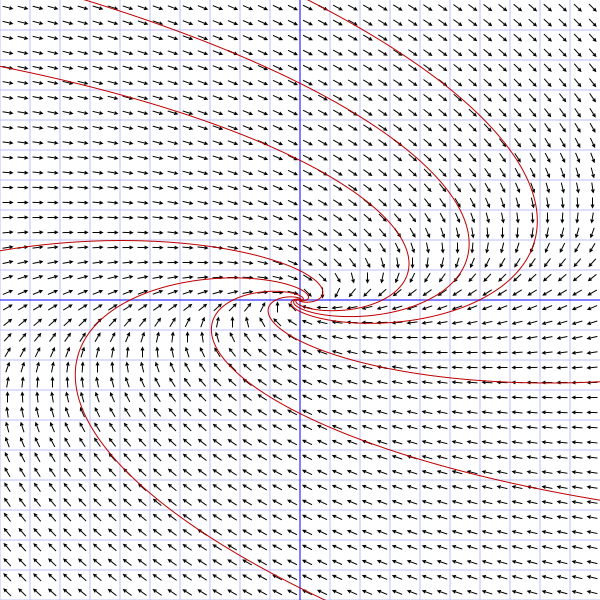
\includegraphics[width=.7\textwidth]{./images/fases-pols.png}
  \end{figure}
\end{enumerate}

\subsection{El primer método de Lyapunov}

Sea $D \subset \R^d$ abierto y $f \in \mathcal{C}^1(D, \R^d)$. Sea $p \in D$ tal que $f(p) = 0$. La
ecuación \eqref{eq:edo:ae} puede escribirse de la forma
\begin{equation}
  \label{eq:3}
  x' = f'(p)x - f'(p)p + R(x),
\end{equation}
con $||R(x)|| / ||x-p|| \to 0$ cuando $x\to p$.

\begin{theorem}[Primer método de Liapunov]
  \label{thm:lyapunov}
  Sea $D \subset \R^d$ abierto y $f \in \mathcal{C}^1(D, \R^d)$. Consideramos la ecuación
  \eqref{eq:edo:ae}.  Sea $p \in D$ con $f(p) = 0$. Sea
  $\mu = \max \{\mathrm{Re}(\lambda) \mid \lambda \in \sigma(f'(p))\}$.
  \begin{enumerate}
  \item Si $\mu < 0$, entonces $p$ es asintóticamente estable.
  \item Si $\mu > 0$, entonces $p$ es inestable.
  \end{enumerate}
\end{theorem}

\begin{ex}
  
  \begin{enumerate}
  \item Consideramos la EDO $x' = -x^3$. El único punto de equilibrio es $p = 0$, que es un atractor
    global. Nótese que $\mu = 0$ y el sistema es asintóticamente estable.
  \item Consideramos la EDO $x' = x^3$. El único punto de equilibrio es $p = 0$, que es un repulsor
    global. Nótese que $\mu = 0$ y el sistema es inestable.
  \item Consideramos la EDO \eqref{eq:edo:ae} asociada a $f(x) = x^3 \sin(1/x)$. Existe una sucesión
    $\{p_n\}$ de puntos de equilibrios convergentes a $0$. Por tanto, $0$ es estable pero no
    asíntóticamente estable.
  \end{enumerate}
\end{ex}

\begin{corollary}
  Si $d = 2$, en el contexto del Teorema \ref{thm:lyapunov} se verifican las siguientes
  afirmaciones.
  \begin{enumerate}
  \item Si $\det(f'(p)) > 0$ y $\mathrm{traza}(f'(p)) < 0$, entonces $p$ es asintóticamente estable
    para $x' = f(x)$.
  \item Si $\det(f'(p)) < 0$ o $\mathrm{traza}(f'(p)) > 0$, entonces $p$ es inestable.
  \end{enumerate}
\end{corollary}

\begin{ex}[Examen final, 2017]
  Dado el sistema cooperativo
  \begin{equation}
    \label{eq:cooperativo}
    \begin{cases}
      x' = (100 − 20 x + 10 y)x;\\
      y' = (300 + 10 x − 30 y)y.
    \end{cases}
  \end{equation}
  \begin{enumerate}
  \item \textbf{Calcula los puntos de equilibrio.} Tenemos que
    $f(x,y) = ((100-20x+10y)x, (300+10x-30y)y)$. Es fácil ver que los únicos ceros de $f$ son
    $\{(0,0), (0,10), (5,0), (12,14)\}$.
  \item \textbf{Estudia las propiedades de estabilidad de los puntos de equilibrio.} Nótese que la
    matriz jacobiana de $f$ viene dada por
    \[ f'(x,y) = \left( \begin{matrix}
          100 -40x +10y & 10x \\
          10x & 300 +10x-60y
        \end{matrix} \right).

    \]
    \begin{itemize}
    \item En $(0,0)$ tenemos $\mathrm{traza}(f'(0,0)) > 0$, luego es inestable.
    \item En $(0,10)$ se cumple $\det(f'(0,10)) > 0$, luego es inestable.
    \item En $(5,0)$ obtenemos $\det(f'(5,0)) < 0$, luego es inestable.
    \item En $(12,14)$ se tiene $\det(f'(12,14)) > 0$ y $\mathrm{traza}(f'(12,14)) < 0$, por lo que
      el punto de equilibrio es asintóticamente estable. \qedhere
    \end{itemize}
  \end{enumerate}
\end{ex}


\end{document}


